\documentclass[letterpaper,landscape]{slides}
%\documentclass[letterpaper,portrait]{slides}
\usepackage{boxedminipage}

%\input /u/rhl/TeX/pdf.tex
\input pdf.tex

\newif\ifTalk\Talktrue		% We generating a talk, not printing
%\Talkfalse			% no; we're really printing

%\pagestyle{empty}
\setlength{\topmargin}{-1in}
\setlength{\textheight}{7.5in}
\setlength{\textwidth}{9in}
\setlength{\oddsidemargin}{0pt}
\setlength{\oddsidemargin}{0pt}

%\onlyslides{1-3,4,10-9999}
%\onlyslides{26-9999}

\begin{document}

\newcommand{\XXX}[1]{\textbf{XXX} #1}
\newcommand{\colour}[1]{\color{#1}}

\def\eq#1{\begin{equation} \color{blue} #1 \end{equation}}

\def\b#1{{\bf  #1}}
\def\p{\partial}
\def\th{^{th}}
\def\msun{{\rm\,M_\odot}}
\def\bnabla{{\bf\nabla}}
\def\dint{\int\!\!\!\int}
\def\d{{\rm d}}
\def\i{{\rm i}}
\def\ddt#1{{\rm{d} #1\over {\rm dt}}}
\def\ddtS#1{{\rm{d^2} #1\over {\rm dt^2}}}
%\lta and \gta produce > and < signs with twiddle underneath
\def\spose#1{\hbox to 0pt{#1\hss}}
\def\lta{\mathrel{\spose{\lower 3pt\hbox{$\mathchar"218$}}
     \raise 2.0pt\hbox{$\mathchar"13C$}}}
\def\gta{\mathrel{\spose{\lower 3pt\hbox{$\mathchar"218$}}
     \raise 2.0pt\hbox{$\mathchar"13E$}}}
\def\mspace{\hbox{\quad}}

\def\deffn#1{{\bf#1}}\def\eqs#1{equations \rf#1}


\newcount\itemCnt\itemCnt=0
\newcommand{\nitem}{%
  \global\advance\itemCnt by 1
  ~\vskip0cm\the\itemCnt.\qquad}

\definecolor{orange}{rgb}{1.0, 0.5, 0.0}
\definecolor{purple}{cmyk}{0.4, 0.8, 0.3, 0.0}


%%%%%%%%%%%%%%%%%%%%%%%%%%%%%%%%%%%
\newcommand{\onepic}[6]{%
\begin{slide}
     \begin{center}
        \begin{minipage}{#1in}
            {\large \color{blue} #6}
            \phantom{x} \vskip #2in
            \phantom{x} \hskip #3in
            {\scalebox{#4}{\includegraphics{#5}}}   
        \end{minipage}
     \end{center}
    \vfill
\end{slide}
}


%%%%%%%%%%%%%%%%%%%%%%%%%%%%%%%%%%%
\newcommand{\picslide}[7]{%
  \begin{slide}
     \begin{center}
        \begin{minipage}{#5in}
            \hskip #6in
            \hskip -1in
            {\scalebox{#4}{\includegraphics{#1.#2}}}
            \vskip #7in~
            {\large \color{blue} #3}
        \end{minipage}
     \end{center}
     \vfill
  \end{slide}
}
%%%%%%%%%%%%%%%%%%%%%%%%%%%%%%%%%%%
 

%%%%%%%%%%%%%%%%%%%%%%%%%%%%%%%%%%%
\newcommand{\Spicslide}[7]{%
  \begin{slide}
     \begin{center}
        \begin{minipage}{#5in}
            \vskip #6in
            \hskip #7in
            {\scalebox{#4}{\includegraphics{#1.#2}}}
        \end{minipage}
     \end{center}
     \vfill
  \end{slide}
}
%%%%%%%%%%%%%%%%%%%%%%%%%%%%%%%%%%%
 

%------------------------------------------------------------------------------
%------------------------------------------------------------------------------

\begin{slide}

\phantom{x}
\vskip -2in
\begin{center}
\bfseries
{\large {\color{blue} Astr 511: Galaxies as galaxies}}
\end{center}

{\centerline {{\color{blue} 
Winter Quarter 2017, University of Washington}}}
{\centerline {{\color{blue} 
Mario Juri\'{c} \& \v{Z}eljko Ivezi\'{c} }}}

\vskip 1.6in

{\centerline {\huge {\color{red}      Lecture 2:             }}}
\vskip 0.2in 
{\centerline {\Large {\color{blue} Basic properties of the Milky Way }}}
{\centerline {\Large {\color{blue} and the Local Group  }}}

\vfill
\end{slide}

%------------------------------------------------------------------------------
%------------------------------------------------------------------------------

\begin{slide}
\begin{center}
{\large \color{red} 
                         Outline
}
\end{center}

\begin{itemize}
\item {\color{blue} Spatial distribution of stars:} disk, halo, bulge
\item {\color{blue} Stellar kinematics:} rotation vs. random motions
\item {\color{blue} Galactic center:} black hole measurements
\item {\color{blue} Interstellar medium:} gas and dust
\item {\color{blue} Stellar counts:} simple analysis
\item {\color{blue} The Local Group:} our nearest galaxy neighborhood 

\end{itemize}          

%{\bf Good sites:}
%http://seds.lpl.arizona.edu/messier/more/mw.html
%http://www.space.com/milkyway

\vfill
\end{slide}


%------------------------------------------------------------------------------
% TWO-SIDED PAGE 
\begin{slide}

\hbox to \hsize{
\begin{minipage}[t]{11.5cm}
\begin{center}
\vskip -0.6in
\scalebox{0.6}{\hskip -1.7in 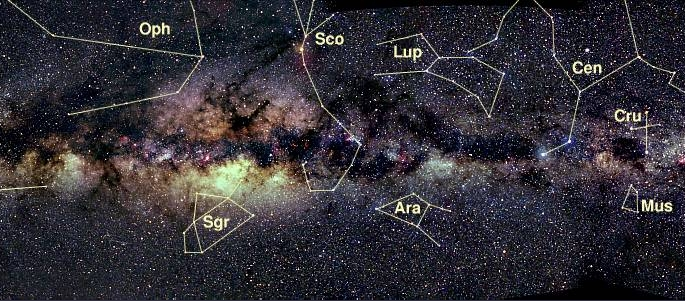
\includegraphics{figures/mljecniput.jpg}}
\vskip 0.1in
\scalebox{0.3}{\hskip  -3.5in 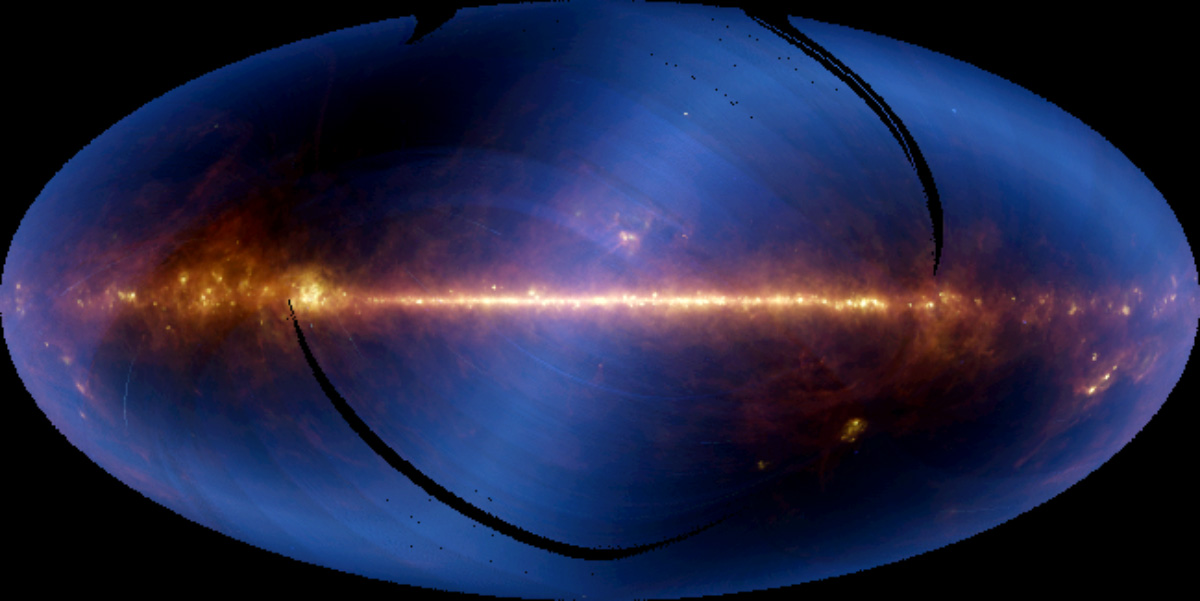
\includegraphics{figures/IRAS_allsky_big.jpg}}
\vskip 0.1in
\scalebox{0.4}{\hskip  -2.6in 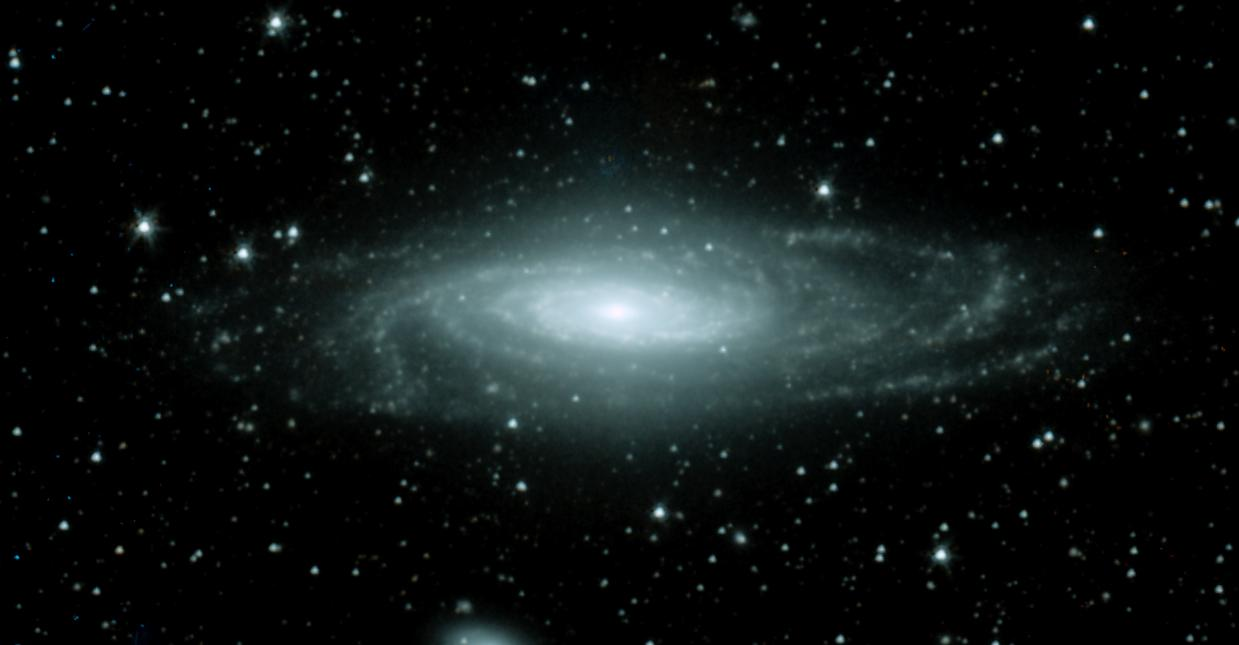
\includegraphics{figures/NGC_7331.jpg}}
\end{center}

\end{minipage}

\begin{minipage}[t]{12.5cm}
\begin{center}
\vskip -1in
{\large \color{red} Introduction }
\end{center}

\begin{itemize}
\item {\color{blue} Top left:} 30$^\circ$ by 10$^\circ$ (optical) view towards
  the Galactic center (from Axel Mellinger)
\item {\color{blue} Middle left:} The all-sky view by the Infrared
                                  Astronomical Satellite
\item {\color{blue} Bottom left:} a spiral galaxy (NGC 7331) similar to the
                                  Milky Way
\item {\color{red} Conclusion:} the density of stars on the sky varies greatly
                    because we are observing from inside a disk of stars
\item {\color{blue} We live in a a spiral galaxy} the same conclusion
           supported by the motions of stars and the presence of abundant 
           interstellar medium (more later)
\end{itemize}

\end{minipage}}
\vfill 
\end{slide}
%--------------------------------------------------------------------------------------------


%------------------------------------------------------------------------------
% TWO-SIDED PAGE 
\begin{slide}

\hbox to \hsize{
\begin{minipage}[t]{6cm}
\begin{center}

\vskip 1.1in
\scalebox{0.7}{\hskip -1.3in 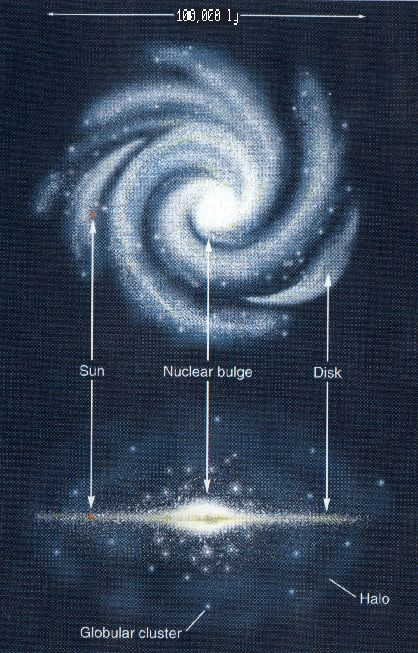
\includegraphics{figures/mw.jpg}}


\end{center}
\end{minipage}

\begin{minipage}[t]{17cm}
\begin{center}
\vskip -1in
{\large \color{red} The position of the Galactic center}
\end{center}


\begin{itemize}
\item
{\color{blue} Shapley used the distribution of globular clusters to
demonstrate that the Sun is not in the center of the Milky Way (8 kpc)} 
\end{itemize}

\vskip 1in
\scalebox{0.7}{\hskip 1.3in 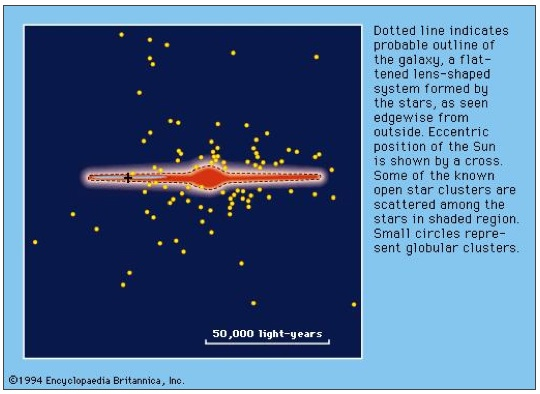
\includegraphics{figures/gc_galaxy.jpg}} 

\end{minipage}}
\vfill 
\end{slide}
%--------------------------------------------------------------------------------------------



%------------------------------------------------------------------------------
% TWO-SIDED PAGE 
\begin{slide}

\hbox to \hsize{
\begin{minipage}[t]{12cm}
\begin{center}
\vskip -6.6in
\scalebox{0.9}{\hskip -1.0in 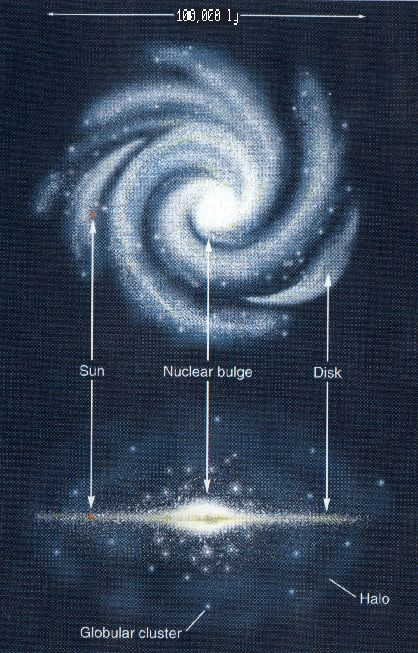
\includegraphics{figures/mw.jpg}}
\end{center}

\end{minipage}

\begin{minipage}[t]{12cm}
\begin{center}
\scalebox{0.8}{\hskip -0.1in 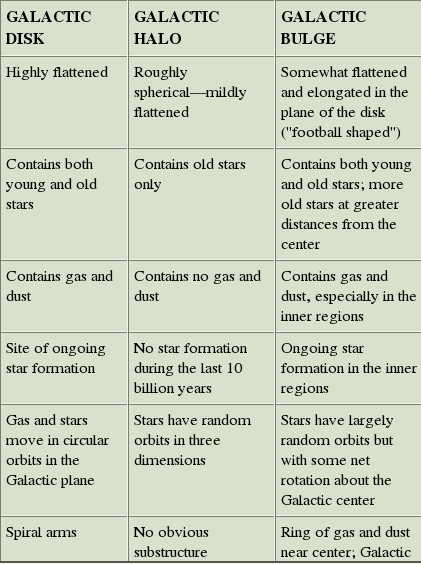
\includegraphics{figures/table.jpg}}
\end{center}

\end{minipage}}
\vfill 
\end{slide}
%--------------------------------------------------------------------------------------------


%------------------------------------------------------------------------------
% TWO-SIDED PAGE 
\begin{slide}

\hbox to \hsize{
\begin{minipage}[t]{8cm}
\begin{center}
\vskip -0.8in
\scalebox{0.6}{\hskip -1.5in 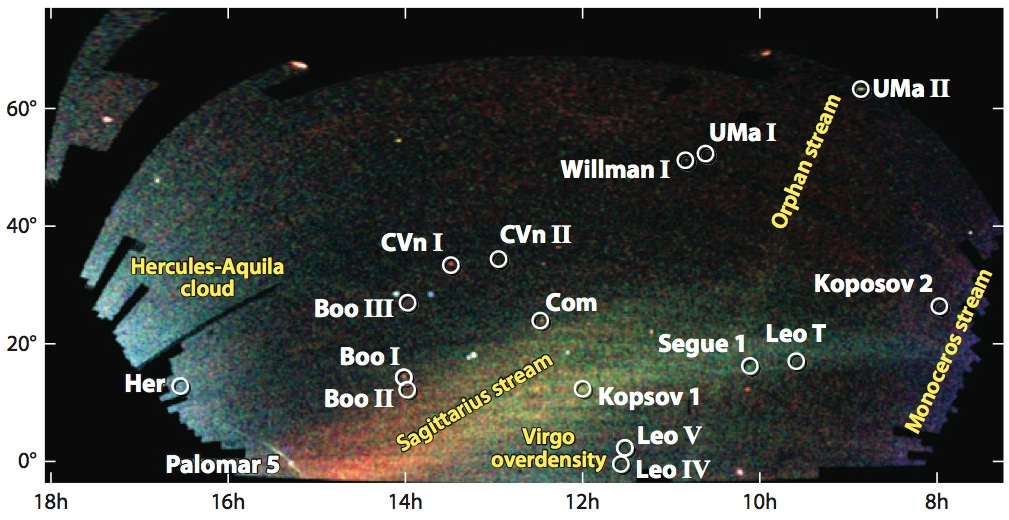
\includegraphics{figures/field_of_streams.jpg}}
\vskip -0.0in
\scalebox{0.42}{\hskip -1.85in 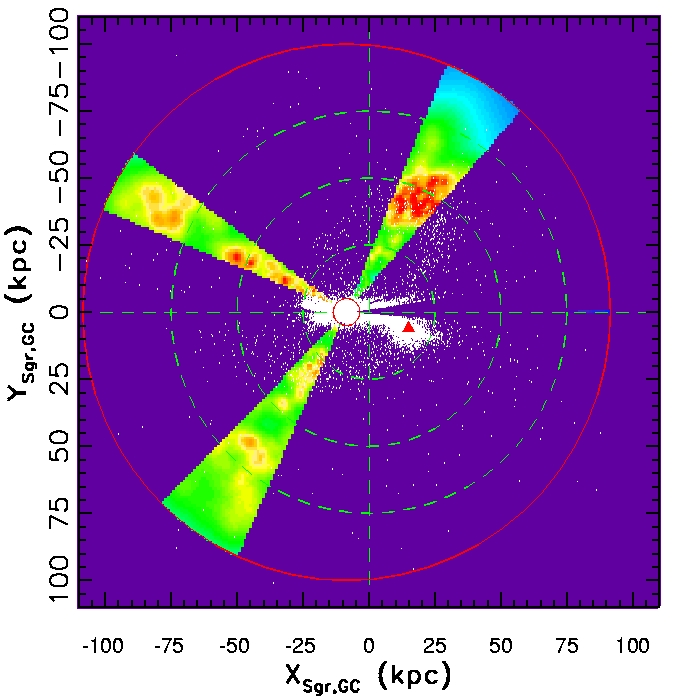
\includegraphics{figures/SgrPlane.jpg}}
\end{center}

\end{minipage}

\begin{minipage}[t]{16cm}
\begin{center}
\vskip 1.1in
{\large \color{red} \,\,\,\,\,\,\,\,\,\,\,\,\,\,\,\,\,\,\,\,\,\,\,\,\,\,\,\,\,\, Halo Substructure }
\end{center}

\vskip 0.1in
\begin{itemize}
\item {\color{blue} The table on the previous page is wrong:} most recent
          data clearly show that {\bf halo has rich substructure}
\item {\color{blue} Top left:} the counts of SDSS stars color-coded by distance
                 (red: $\sim$10 kpc, blue: several kpc) from Belokurov et al. (2007)
\item {\color{blue} Bottom left:} the distribution of SDSS RR Lyrae stars
                 and 2MASS red giants (Ivezi\'{c} et al. 2003)
\end{itemize}

\end{minipage}}
\vfill 
\end{slide}
%--------------------------------------------------------------------------------------------


%------------------------------------------------------------------------------
% TWO-SIDED PAGE 
\begin{slide}

\hbox to \hsize{
\begin{minipage}[t]{1cm}
\begin{center}
\vskip 2.9in
\scalebox{0.8}{\hskip -0.9in 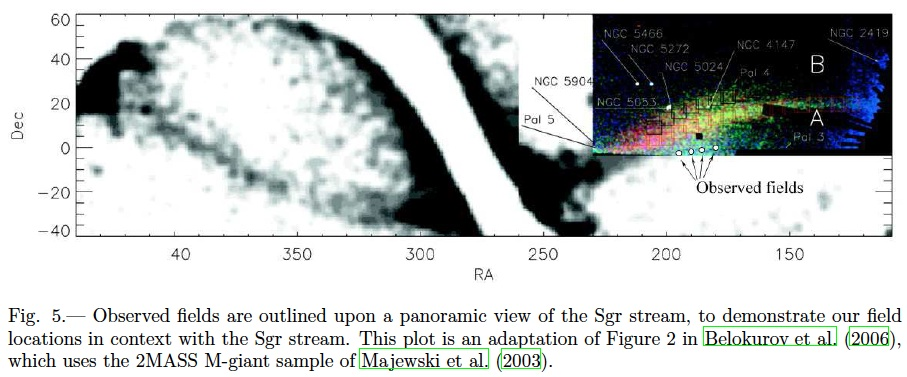
\includegraphics{figures/SgrStreamPanoramic_Casey2012.jpg}}
\end{center}
\end{minipage}

\begin{minipage}[t]{20cm}
\begin{center}
\vskip -1in
{\large \color{red} The Virgo Overdensity: the latest news}
\end{center}
\vskip 0.2in
\begin{itemize}
\item ``...the Virgo Overdensity ... is best explained by a minor merger.''
(Bonaca et al. 2012, AJ 143, 105), 
\item
``... a tri-axial dark matter halo is favored and we exclude a prolate shape.''
(Casey, Keller \& Da Costa 2012, AJ 143, 88; figure below is from this paper)
\end{itemize}  


\end{minipage}}
\vfill 
\end{slide}
%--------------------------------------------------------------------------------------------



%------------------------------------------------------------------------------
% TWO-SIDED PAGE 
\begin{slide}

\hbox to \hsize{
\begin{minipage}[t]{10cm}
\begin{center}
\vskip -0.75in
\scalebox{0.05}{\hskip -10.4in \includegraphics{figures/MWplaneAnnotated.jpg}}
\vskip 0.1in
\scalebox{0.37}{\hskip -2.8in 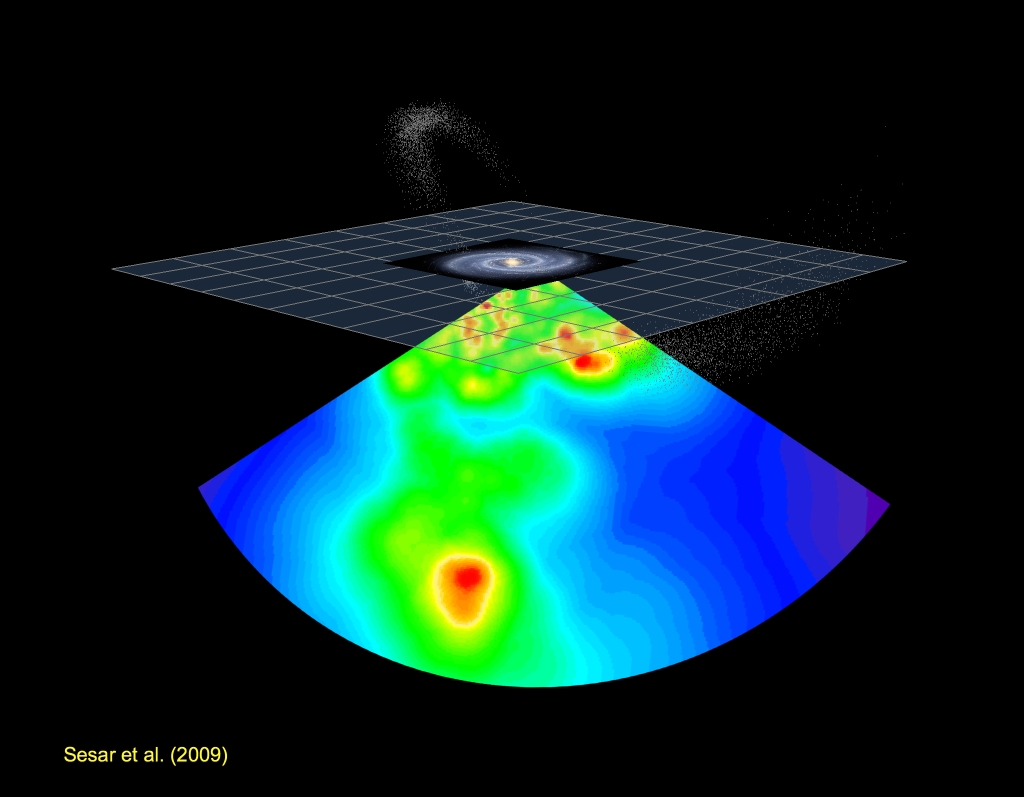
\includegraphics{figures/snapshot1.jpg}}
\end{center}
\end{minipage}

\begin{minipage}[t]{14cm}
\begin{center}
\vskip -1in
{\large \color{red} Outer halo studies: RR Lyrae (from SDSS)}
\end{center}

\begin{itemize}
\item {\bf Top left:} the disk structure (artist's conception based on the Spitzer and
      other surveys of the Galactic plane)
\item {\bf Bottom left:} the halo density (multiplied by $R^3$; yellow and red are overdensities
      relative to mean $\rho(R)\propto R^{-3}$ density) as traced by RR Lyrae from SDSS Stripe 82
      (Sesar et al. 2010ab, ApJ 708, 717; ApJ 717, 133), compared in scale to the top panel
\item {\color{blue} Conclusions:} the spatial distribution of halo stars is highly
inhomogeneous (clumpy); when averaged, the stellar volume density decreases
as $\rho(R)\propto R^{-3}$ out to $\sim$30 kpc, and then becomes steeper.
\end{itemize}     

\end{minipage}}
\vfill 
\end{slide}
%------------------------------------------------------------------------------





%------------------------------------------------------------------------------
% TWO-SIDED PAGE 
\begin{slide}

\hbox to \hsize{
\begin{minipage}[t]{10cm}
\begin{center}
\vskip -0.6in
\scalebox{1.1}{\hskip -1.6in 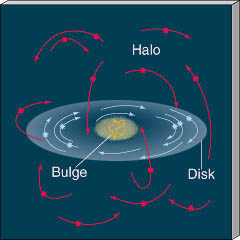
\includegraphics{figures/motion.jpg}}
\vskip 0.1in
\scalebox{0.9}{\hskip -1.5in 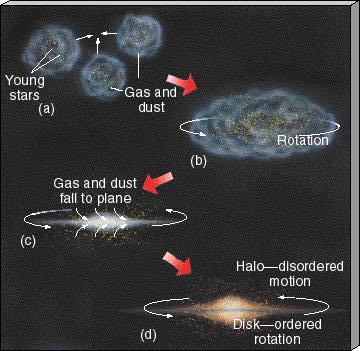
\includegraphics{figures/formation.jpg}}
\end{center}

\end{minipage}

\begin{minipage}[t]{14cm}
\begin{center}
{\large \color{red} Kinematics }
\end{center}


\begin{itemize}
\item {\color{blue} Stars move} in a gravitational potential (more in L13)
\item {\color{blue} Two types of motion:} disk stars {\bf rotate} around the
  center, while halo stars are on randomly distributed elliptical orbits (more
  in L11) 
\item {\color{blue} The motion of stars was set during the formation period}
\item {\color{red} The details are governed by the laws of physics:}
            conservation of energy and conservation of angular momentum!
\item As the cloud collapses, its rotation speed must increase. As it 
      spins faster, it must flatten.
\end{itemize}

\end{minipage}}
\vfill 
\end{slide}
%------------------------------------------------------------------------------
% TWO-SIDED PAGE 
\begin{slide}

\hbox to \hsize{
\begin{minipage}[t]{9cm}
\begin{center}
\vskip -0.7in
\scalebox{0.4}{\hskip -1.8in 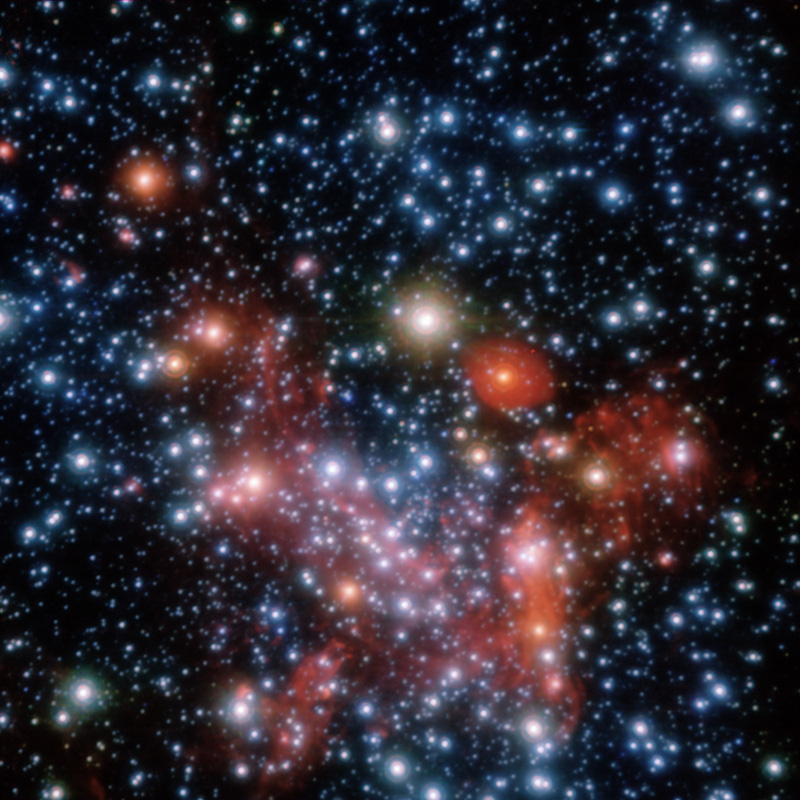
\includegraphics{figures/MWcenter.jpg}}
\vskip 0.1in
\scalebox{0.5}{\hskip -1.6in 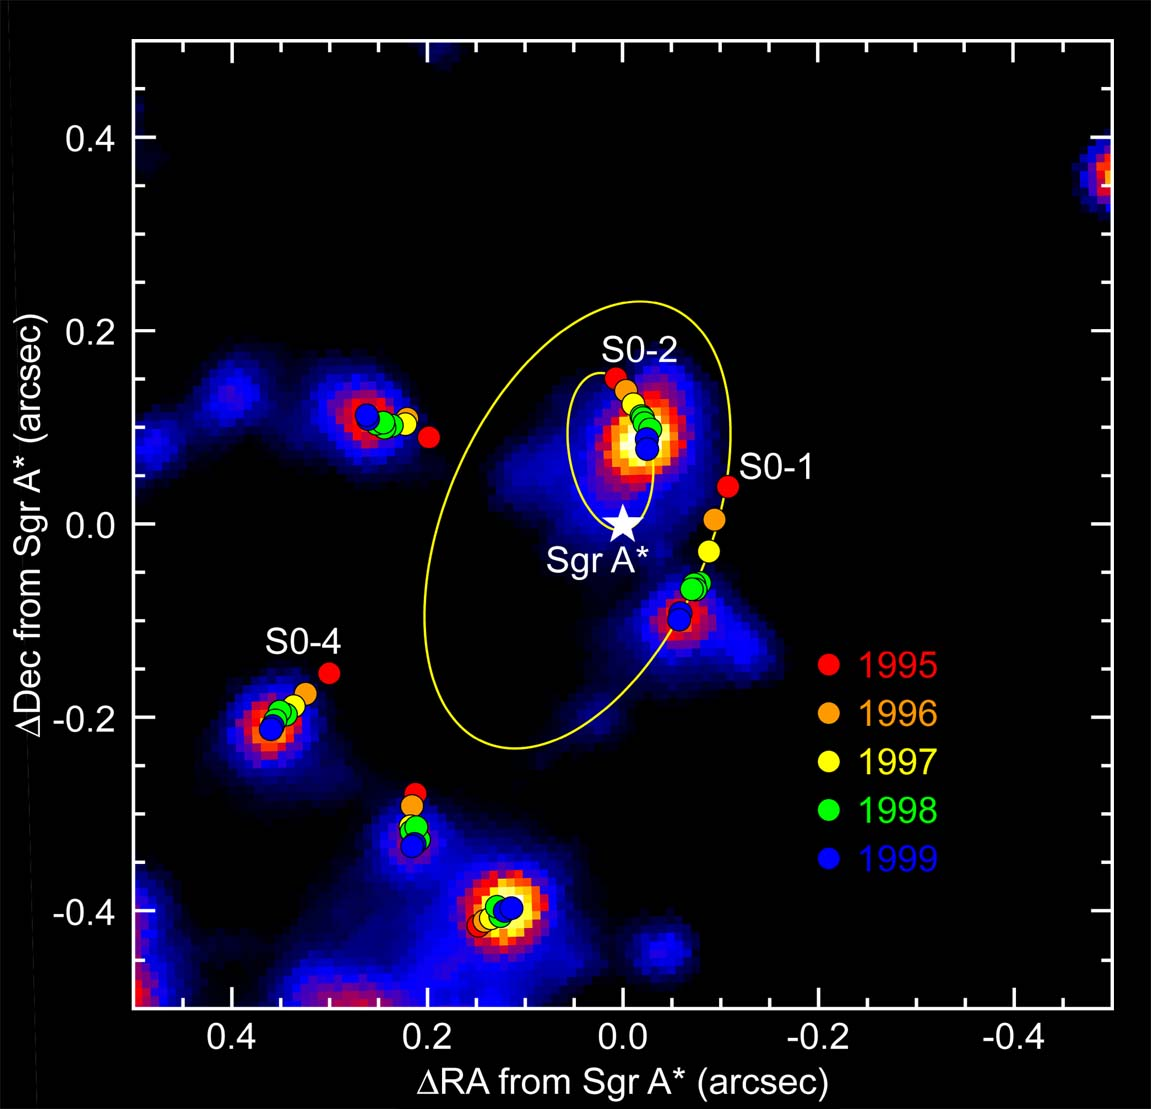
\includegraphics{figures/SgrA_BH.jpg}}
\end{center}

\end{minipage}

\begin{minipage}[t]{15cm}
\begin{center}
\vskip -0.1in \hskip 0.04in
{\large \color{red} \phantom{} Black Hole in the Galactic Center }
\end{center}


\begin{itemize}
\item {\color{blue} Stars move} in a gravitational potential: {\color{blue} 
    a large mass (a few 10$^6$ $M_\odot$) confined to small space (0.1-0.2
    AU)} is required to explain about
    $\sim$30 {\bf observed} orbits
\item Two teams: UCLA team led by Andrea Ghez, and European team led by
   Reinhard Genzel 
\end{itemize}
\vskip 0.3in
\scalebox{2.9}{\hskip 0.06in 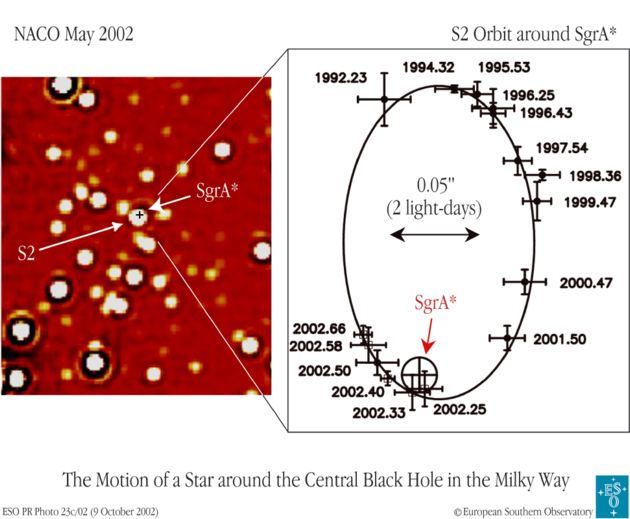
\includegraphics{figures/blackhole1.jpg}}

\end{minipage}}
\vfill 
\end{slide}
%----------------------------------------------------------------------------------

%------------------------------------------------------------------------------
% TWO-SIDED PAGE 
\begin{slide}

\hbox to \hsize{
\begin{minipage}[t]{9cm}
\begin{center}
\vskip 0.1in
\scalebox{0.9}{\hskip -1.1in 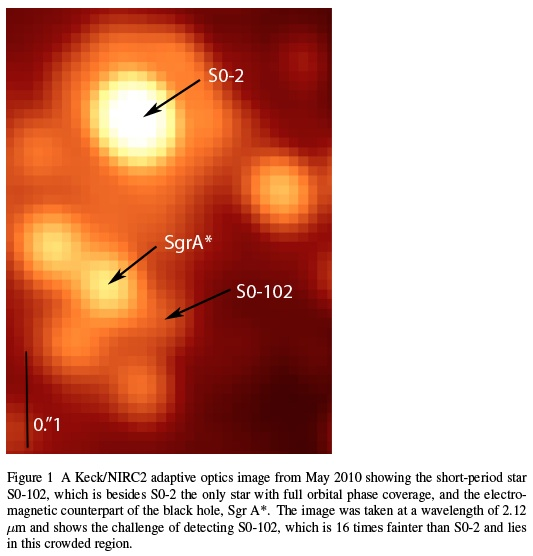
\includegraphics{figures/Ghez_2013_2.jpg}}
\end{center}

\end{minipage}

\begin{minipage}[t]{15cm}
\begin{center}
\vskip -0.1in \hskip 0.04in
{\large \color{red} \phantom{} Black Hole in the Galactic Center }
\end{center}


\begin{itemize}
\item Meyer et al. (2012, Science 338, 84): after 17 years of imaging the galactic center at the highest angular 
resolution possible today: two stars with full phase coverage and periods of less than 20 years. 
\end{itemize}
\vskip 0.1in
\scalebox{0.4}{\hskip 3.6in 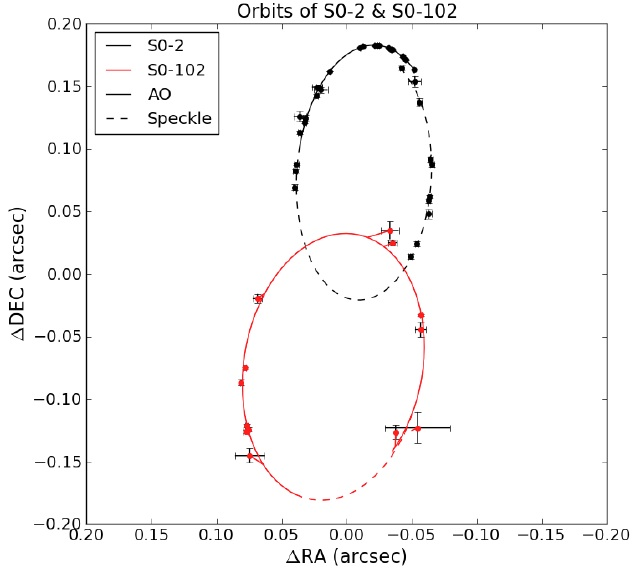
\includegraphics{figures/Ghez_2013_1.jpg}}

\end{minipage}}
\vfill 
\end{slide}
%----------------------------------------------------------------------------------






%------------------------------------------------------------------------------
% TWO-SIDED PAGE 
\begin{slide}

\hbox to \hsize{
\begin{minipage}[t]{12cm}
\begin{center}
\vskip -0.6in
\scalebox{1.1}{\hskip -1.0in 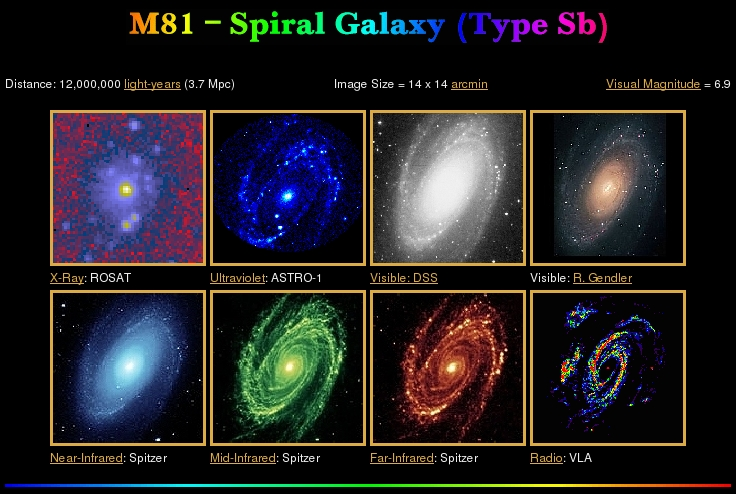
\includegraphics{figures/M81_multiLambda.jpg}}
\end{center}

\end{minipage}

\begin{minipage}[t]{12cm}
\begin{center}
%{\large \color{red} ISM Medium }
\end{center}


\end{minipage}}
\vfill 
\end{slide}
%--------------------------------------------------------------------------------------------



%------------------------------------------------------------------------------
% TWO-SIDED PAGE 
\begin{slide}

\hbox to \hsize{
\begin{minipage}[t]{13cm}
\begin{center}
\vskip -0.6in
\phantom{xx}
\scalebox{0.08}{\hskip -10.4in \includegraphics{figures/MWplaneAnnotated.jpg}}
\end{center}

\end{minipage}

\begin{minipage}[t]{11cm}
\begin{center}
\vskip -1in
{\large \color{red} \phantom{xx} Revised Spiral Arms }
\end{center}


\begin{itemize}
\item The stellar bar was discovered in 1990s based on IRAS data
\item It was believed that the Galaxy has four spiral arms: the
       Scutum-Centaurus, Perseus, Sagittarius and Norma
\item {\color{blue} The stellar counts from Spitzer}  galactic plane survey
   (Benjamin et al. 2008) strongly suggest that there are only two major arms, 
    the Scutum-Centaurus and Perseus arms, as is common for barred galaxies 
\end{itemize}

\end{minipage}}
\vfill 
\end{slide}
%----------------------------------------------------------------------------------






%------------------------------------------------------------------------------
% TWO-SIDED PAGE 
\begin{slide}

\hbox to \hsize{
\begin{minipage}[t]{12cm}
\begin{center}
\vskip -0.6in
\scalebox{1.1}{\hskip -1.0in 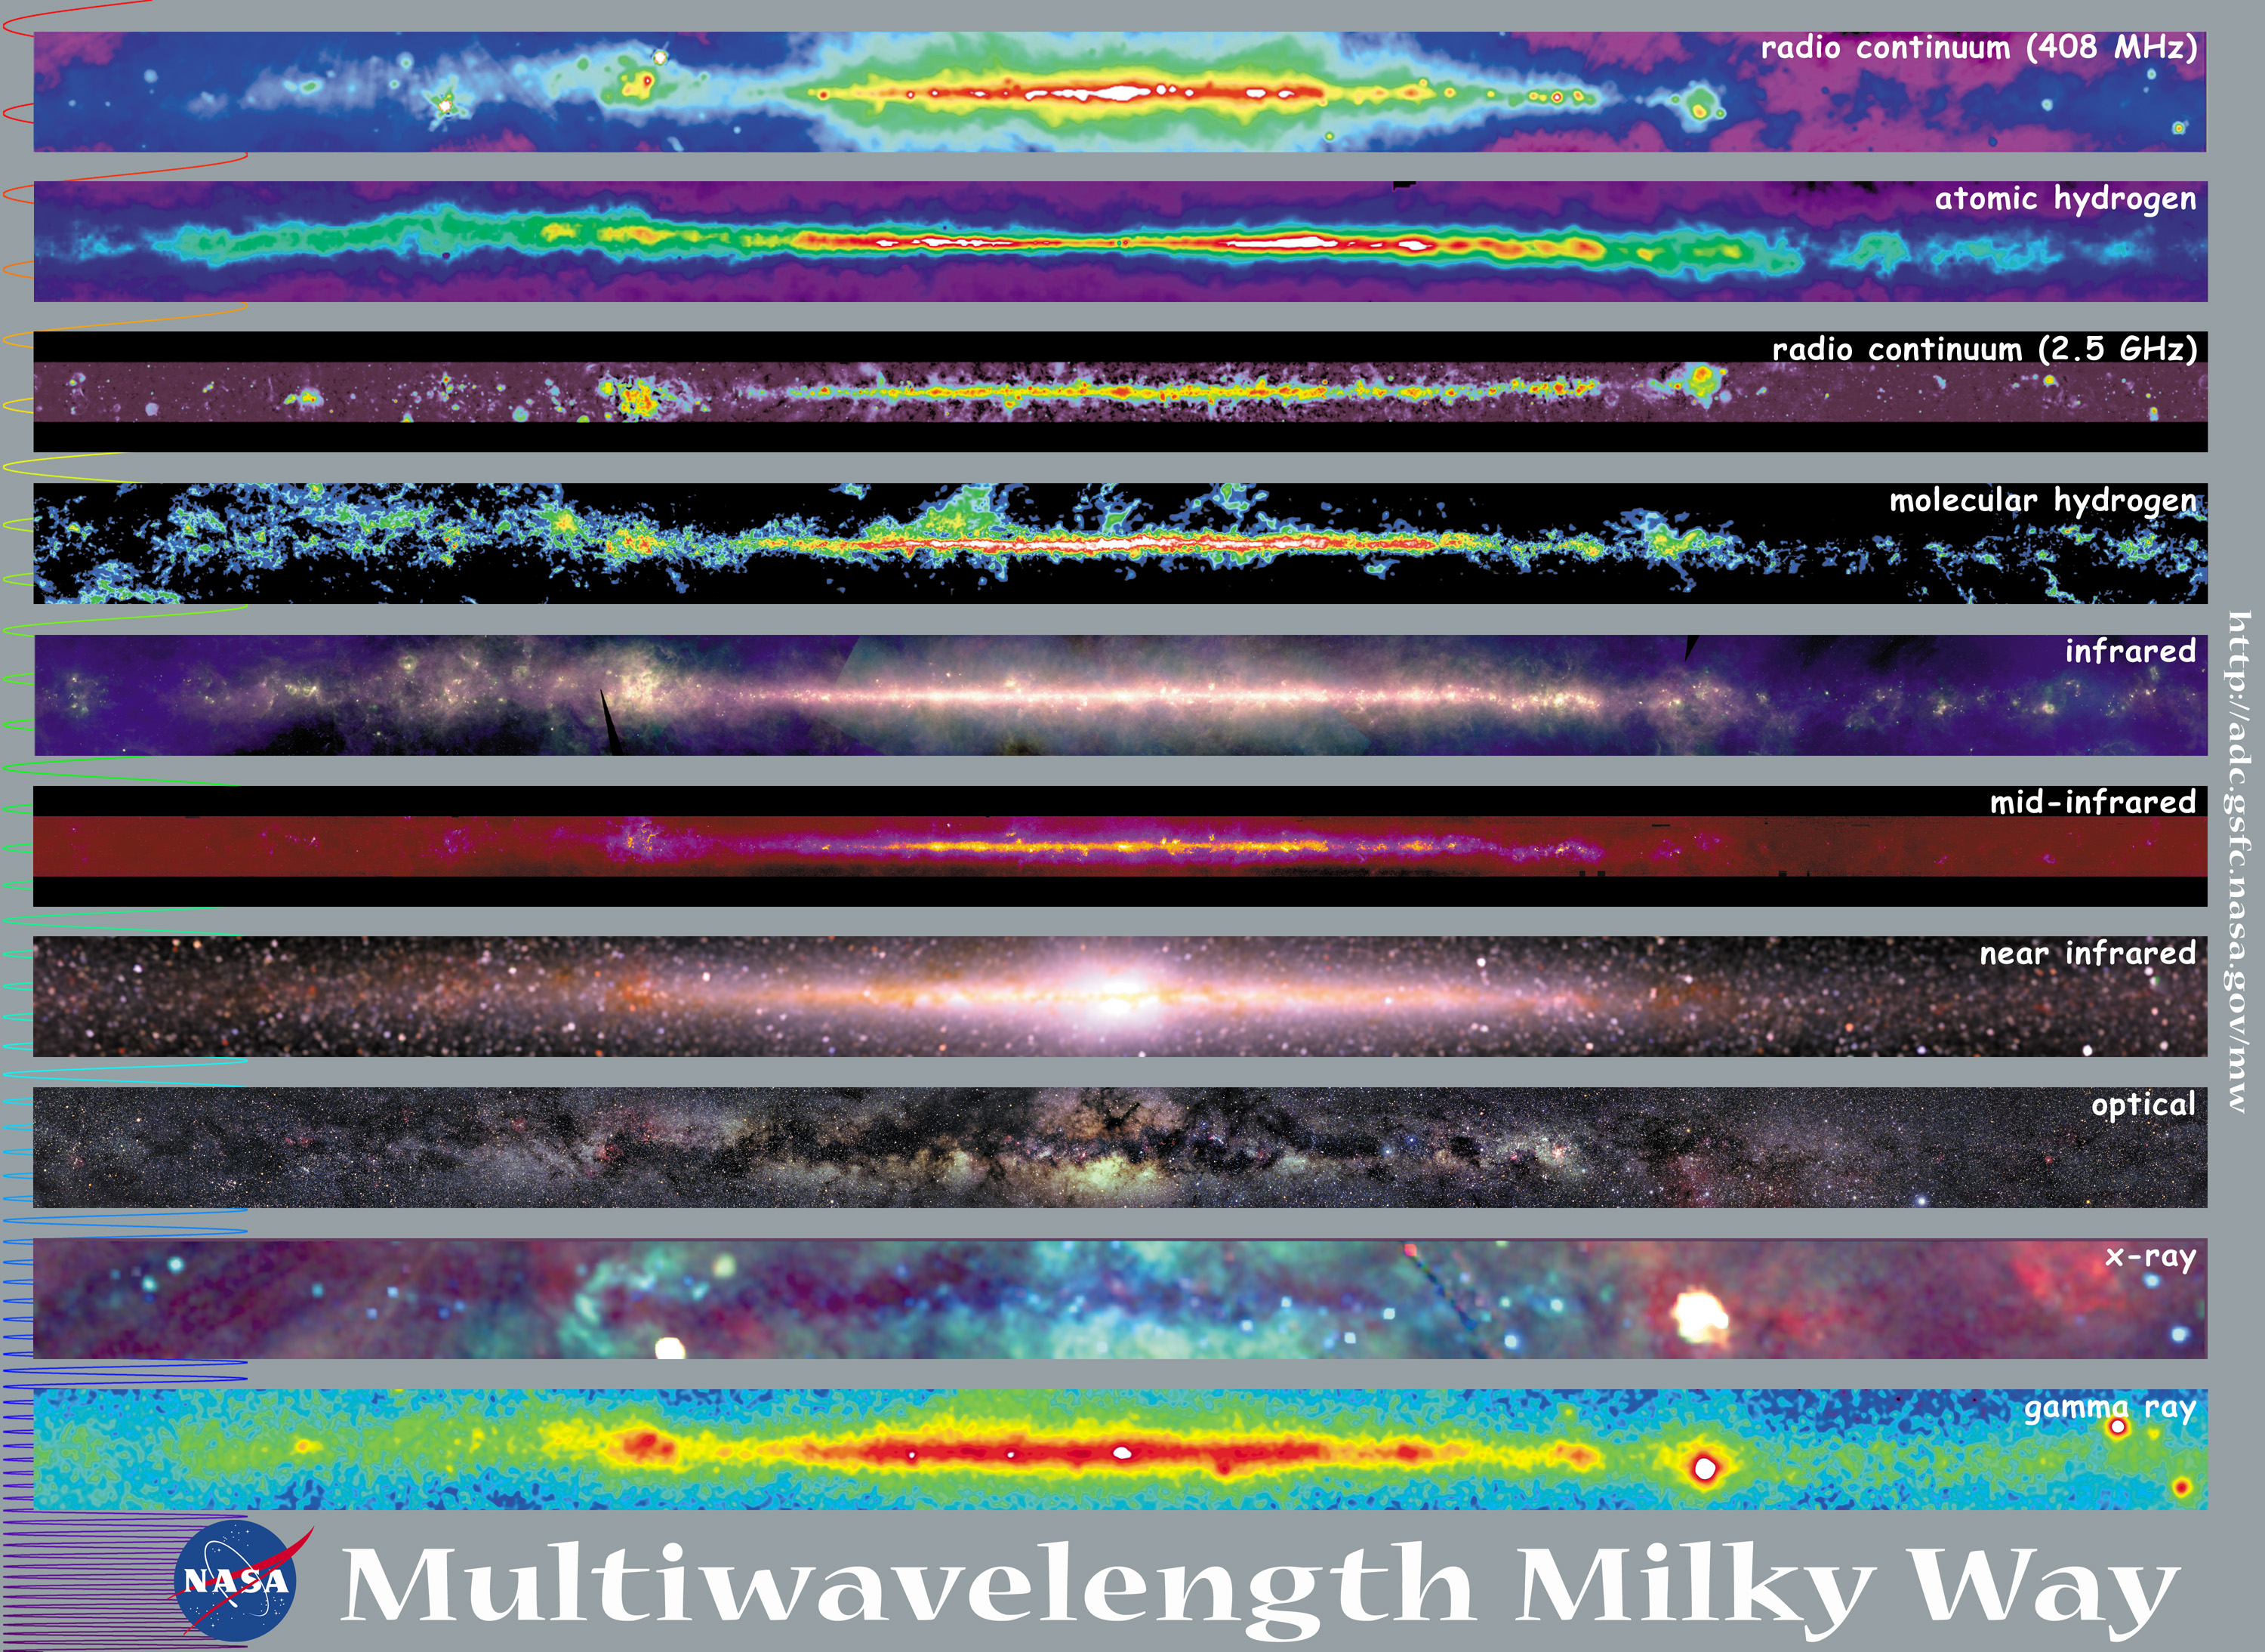
\includegraphics{figures/mwmw_8x10.jpg}}
\end{center}

\end{minipage}

\begin{minipage}[t]{12cm}
\begin{center}
%{\large \color{red} ISM Medium }
\end{center}


\end{minipage}}
\vfill 
\end{slide}
%--------------------------------------------------------------------------------------------




%------------------------------------------------------------------------------
% TWO-SIDED PAGE 
\begin{slide}

\hbox to \hsize{
\begin{minipage}[t]{10cm}
\begin{center}
\vskip -0.1in
\scalebox{1.1}{\hskip -2.7in 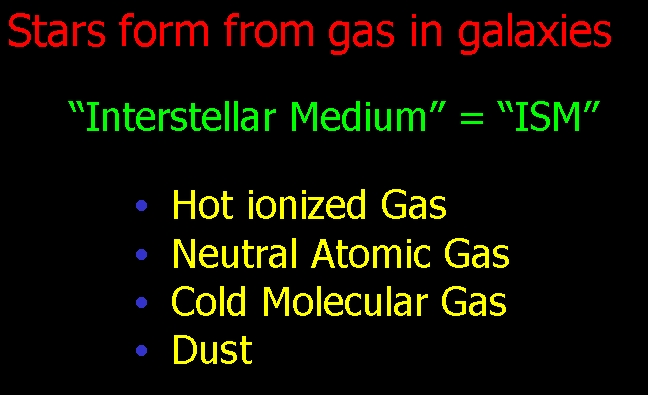
\includegraphics{figures/ISM1.jpg}}
\end{center}
\end{minipage}

\begin{minipage}[t]{14cm}
\end{minipage}}
\vfill 
\end{slide}
%--------------------------------------------------------------------------------------------


%------------------------------------------------------------------------------
% TWO-SIDED PAGE 
\begin{slide}

\hbox to \hsize{
\begin{minipage}[t]{10cm}
\begin{center}
\vskip -0.6in
\scalebox{1.1}{\hskip -3.0in 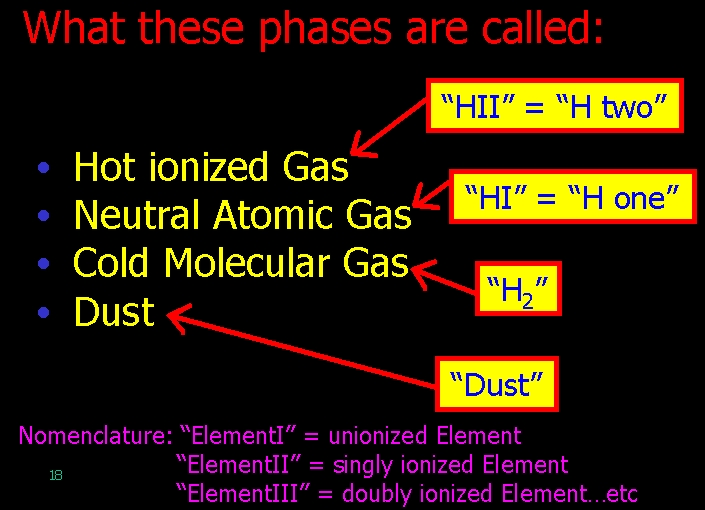
\includegraphics{figures/ISM2.jpg}}
\end{center}
\end{minipage}

\begin{minipage}[t]{14cm}
\end{minipage}}
\vfill 
\end{slide}
%--------------------------------------------------------------------------------------------



%------------------------------------------------------------------------------
% TWO-SIDED PAGE 
\begin{slide}

\hbox to \hsize{
\begin{minipage}[t]{10cm}
\begin{center}
\vskip -0.1in
\scalebox{1.1}{\hskip -2.6in 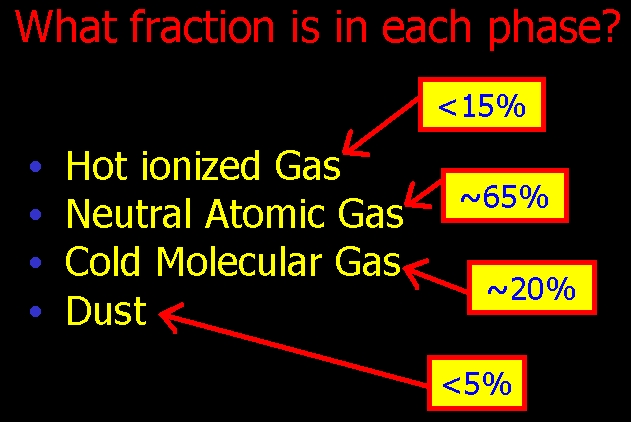
\includegraphics{figures/ISM3.jpg}}
\end{center}
\end{minipage}

\begin{minipage}[t]{14cm}
\end{minipage}}
\vfill 
\end{slide}
%--------------------------------------------------------------------------------------------




%------------------------------------------------------------------------------
% TWO-SIDED PAGE 
\begin{slide}

\hbox to \hsize{
\begin{minipage}[t]{10cm}
\begin{center}
\vskip -0.6in
\scalebox{1.1}{\hskip -2.9in 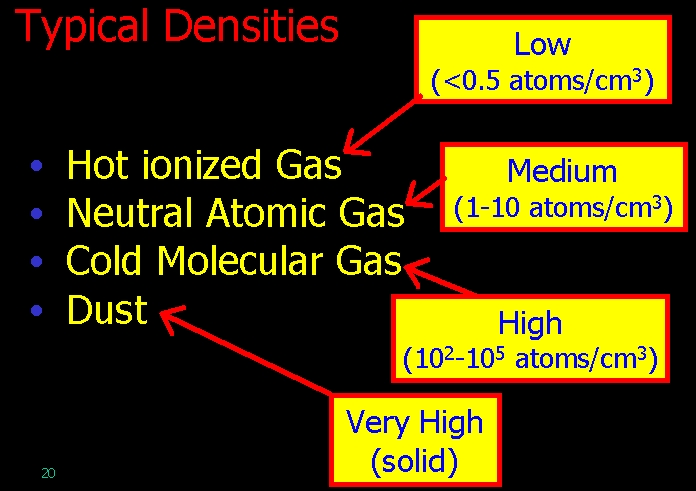
\includegraphics{figures/ISM4.jpg}}
\end{center}
\end{minipage}

\begin{minipage}[t]{14cm}
\end{minipage}}
\vfill 
\end{slide}
%--------------------------------------------------------------------------------------------




%------------------------------------------------------------------------------
% TWO-SIDED PAGE 
\begin{slide}

\hbox to \hsize{
\begin{minipage}[t]{10cm}
\begin{center}
\vskip -0.3in
\scalebox{1.1}{\hskip -2.9in 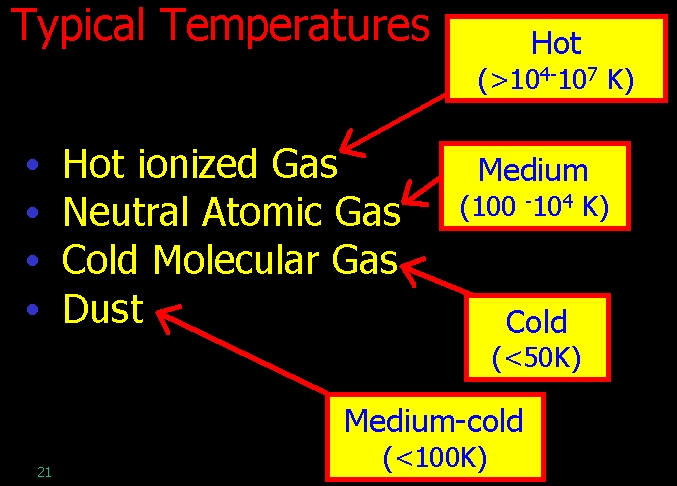
\includegraphics{figures/ISM5.jpg}}
\end{center}
\end{minipage}

\begin{minipage}[t]{14cm}
\end{minipage}}
\vfill 
\end{slide}
%--------------------------------------------------------------------------------------------

%------------------------------------------------------------------------------
% TWO-SIDED PAGE 
\begin{slide}

\hbox to \hsize{
\begin{minipage}[t]{10cm}
\begin{center}
\vskip -0.4in
\scalebox{1.0}{\hskip -2.9in 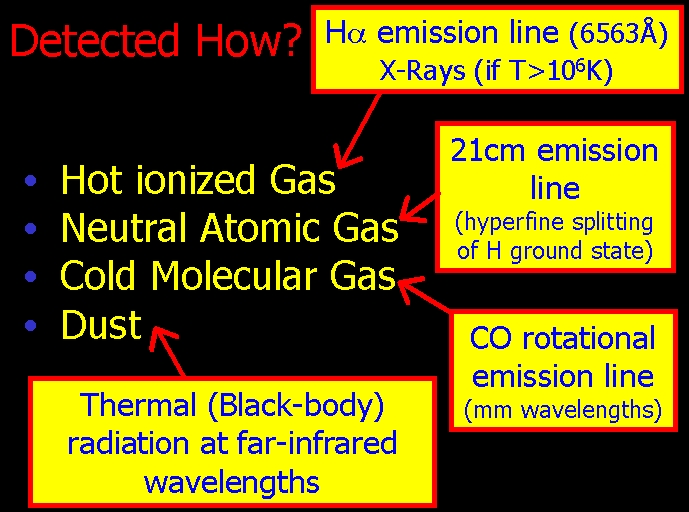
\includegraphics{figures/ISM6.jpg}}
\end{center}
\end{minipage}

\begin{minipage}[t]{14cm}
\end{minipage}}
\vfill 
\end{slide}
%--------------------------------------------------------------------------------------------



%------------------------------------------------------------------------------
% TWO-SIDED PAGE 
\begin{slide}

\hbox to \hsize{
\begin{minipage}[t]{10cm}
\begin{center}
\vskip -0.1in
\scalebox{1.0}{\hskip -2.9in 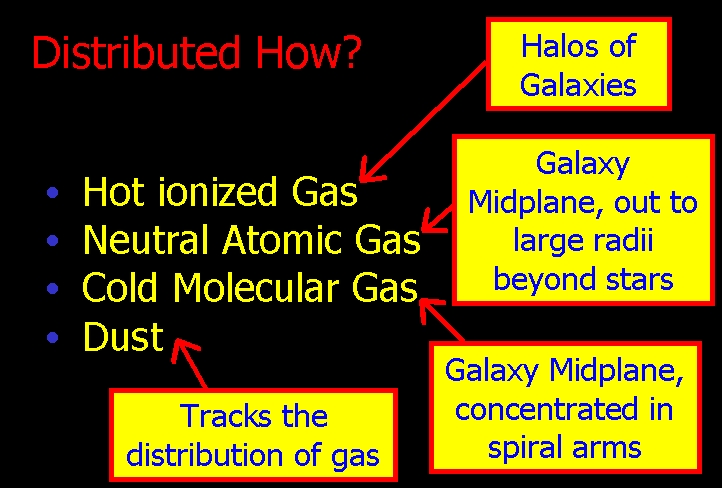
\includegraphics{figures/ISM7.jpg}}
\end{center}
\end{minipage}

\begin{minipage}[t]{14cm}
\end{minipage}}
\vfill 
\end{slide}
%--------------------------------------------------------------------------------------------




%------------------------------------------------------------------------------
% TWO-SIDED PAGE 
\begin{slide}

\hbox to \hsize{
\begin{minipage}[t]{10cm}
\begin{center}
\vskip -0.2in
\scalebox{1.0}{\hskip -0.6in 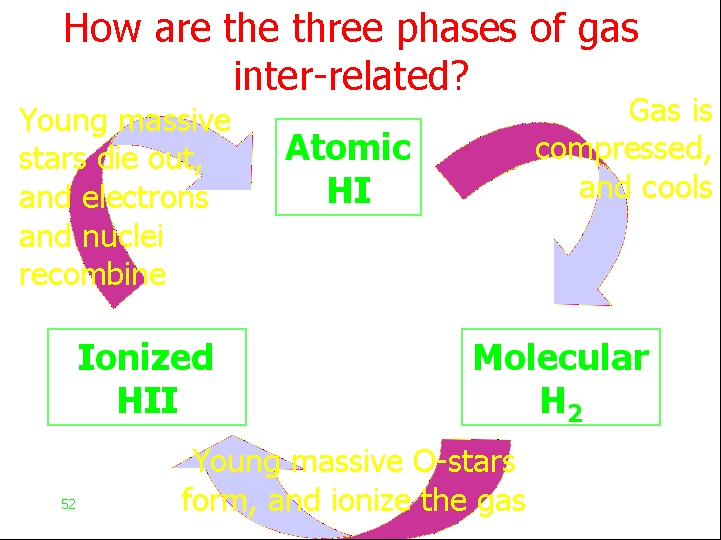
\includegraphics{figures/ISM3phases.jpg}}
\end{center}

\end{minipage}

\begin{minipage}[t]{14cm}
\begin{center}
%{\large \color{red} Interstellar dust }
\end{center}

\end{minipage}}
\vfill 
\end{slide}
%--------------------------------------------------------------------------------------------


%------------------------------------------------------------------------------
% TWO-SIDED PAGE 
\begin{slide}

\hbox to \hsize{
\begin{minipage}[t]{10cm}
\begin{center}
\vskip -0.1in
\scalebox{1.1}{\hskip -1.1in 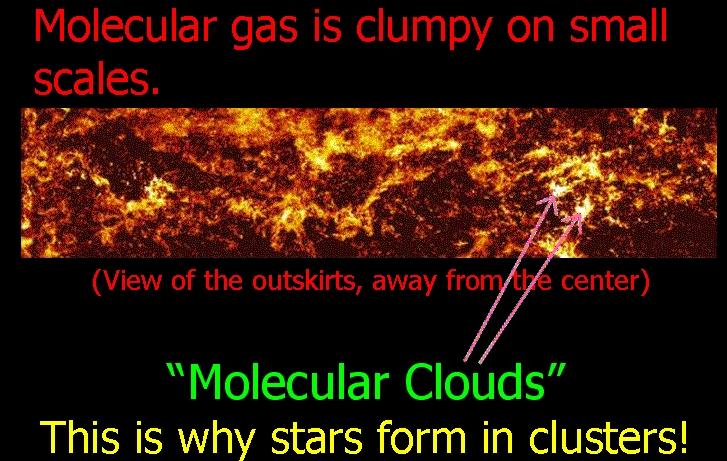
\includegraphics{figures/ISMmolgas.jpg}}
\end{center}

\end{minipage}

\begin{minipage}[t]{14cm}
\begin{center}
%{\large \color{red} Interstellar dust }
\end{center}

\end{minipage}}
\vfill 
\end{slide}
%--------------------------------------------------------------------------------------------



%------------------------------------------------------------------------------

\begin{slide}
\begin{center}
{\large \color{red} A comment about detection of molecular hydrogen}
\end{center}

\begin{itemize}
\item Molecular hydrogen ($H_2$) is hard to detect in ground-based observations 
(optical, near-IR, radio). The reason is that its rotational energy levels are difficult 
to excite in the cold ISM (due to small moment of inertia of H2). 
\item Various tracer molecules, such as carbon monoxide, hydrogen cyanide, ammonia, water, 
and formaldehyde, are used instead to infer the amount of $H_2$ (how do we know that e.g. 
$CO$ is correlated with $H_2$?  See, for example, 	Rachford et al. 2012, ApJ 577, 221). 
\item Nevertheless, {\color{blue} $H_2$ {\bf is} directly detectable:} in the UV via absorbtion
(Copernicus and FUSE space missions, e.g. Richter, Sembach \& Howk 2003, A\&A 405, 1013), 
and in the mid-IR via emission lines (the Spitzer space mission, e.g. Ingalls et al. 2011, 
ApJ 743, 174).
%\item 
%The lowest-lying transitions are the electric quadrupole pure-rotational lines. 
%Because $H_2$ lacks an electric dipole moment, the $J=1$ level is unable to 
%radiate, so the first radiating level is $J = 2$. The first three rotational 
%transitions are $J = 2-0$ at 28.2 $\mu m$, $J = 3-1$ at 17.0 $\mu m$,
%and $J = 4-2$ at 12.3 $\mu m$.
\end{itemize}          

\vfill
\end{slide}






%------------------------------------------------------------------------------
% TWO-SIDED PAGE 
\begin{slide}

\hbox to \hsize{
\begin{minipage}[t]{10cm}
\begin{center}
\vskip -0.6in
\scalebox{1.1}{\hskip -0.8in 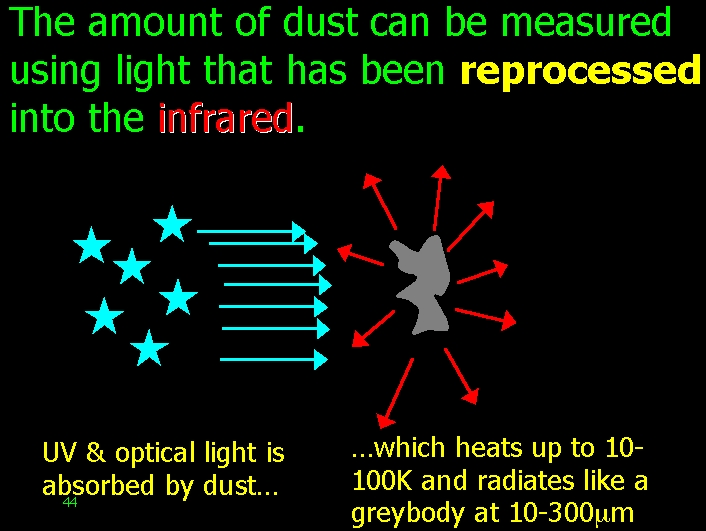
\includegraphics{figures/ISMdust0.jpg}}
\end{center}

\end{minipage}

\begin{minipage}[t]{14cm}
\begin{center}
%{\large \color{red} Interstellar dust }
\end{center}

\end{minipage}}
\vfill 
\end{slide}
%--------------------------------------------------------------------------------------------


%------------------------------------------------------------------------------
% TWO-SIDED PAGE 
\begin{slide}

\hbox to \hsize{
\begin{minipage}[t]{10cm}
\begin{center}
\vskip -0.6in
\scalebox{1.1}{\hskip -1.0in 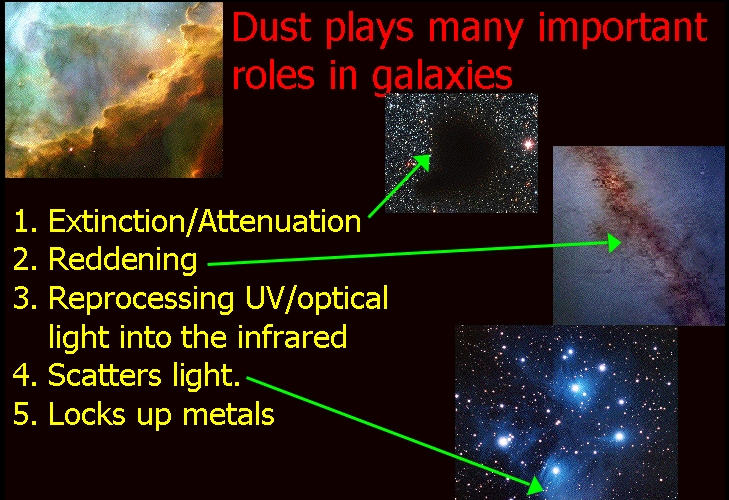
\includegraphics{figures/ISMdust1.jpg}}
\end{center}

\end{minipage}

\begin{minipage}[t]{14cm}
\begin{center}
%{\large \color{red} Interstellar dust }
\end{center}

\end{minipage}}
\vfill 
\end{slide}
%--------------------------------------------------------------------------------------------






%------------------------------------------------------------------------------
% TWO-SIDED PAGE 
\begin{slide}

\hbox to \hsize{
\begin{minipage}[t]{8cm}
\begin{center}
\vskip -0.8in
\scalebox{0.9}{\hskip -1.2in 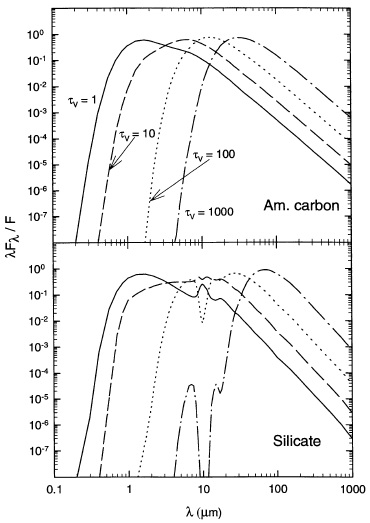
\includegraphics{figures/IE_fig3.jpg}}
%\vskip 0.1in
%\scalebox{0.4}{\hskip  -3.5in 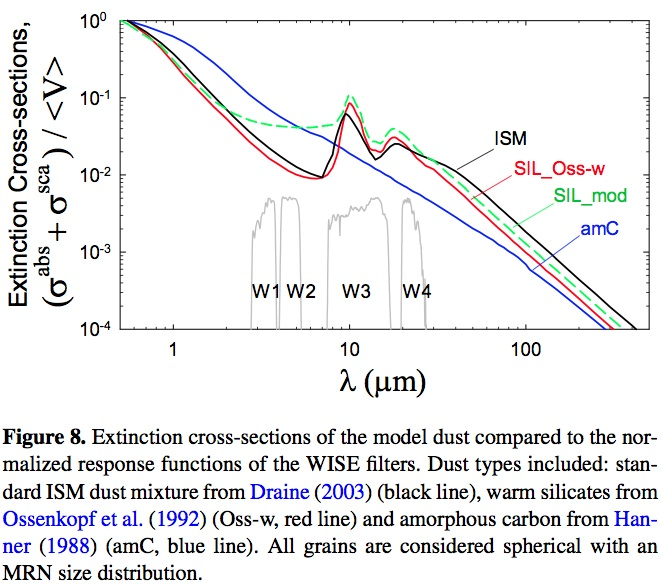
\includegraphics{figures/Nikutta_fig8.jpg}}
\vskip -0.2in
Spectral energy distributions for a star embedded in a spherical 
dusty shell ($\rho(r)\propto 1/r^2$). 
\end{center}

\end{minipage}

\begin{minipage}[t]{15cm}
\begin{center}
\vskip -1in
{\large \color{red} Dust \& radiative transfer}
\end{center}

\begin{itemize}
\item {\color{blue} Left:} radiative transfer modeling (fig. 3 from Ivezi\'{c} \& Elitzur 1997, MNRAS 287, 799)
\item {\color{blue} Below:} modeling of dust optical properties. 
\end{itemize}

\vskip 0.2in
\scalebox{0.6}{\hskip 1.2in 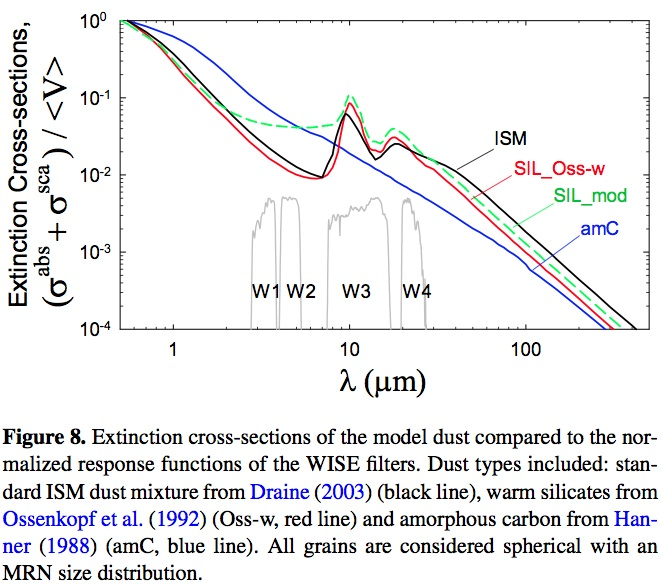
\includegraphics{figures/Nikutta_fig8.jpg}}

\end{minipage}}
\vfill 
\end{slide}
%--------------------------------------------------------------------------------------------





%------------------------------------------------------------------------------
% TWO-SIDED PAGE 
\begin{slide}

\hbox to \hsize{
\begin{minipage}[t]{10cm}
\begin{center}
\vskip -0.6in
\scalebox{1.1}{\hskip -1.1in 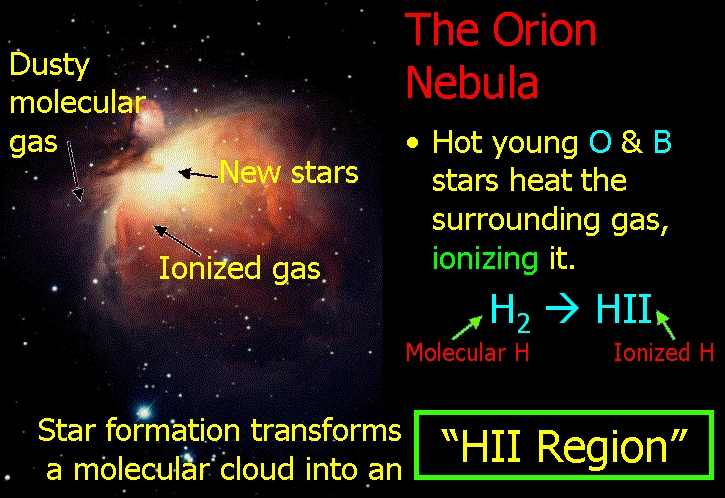
\includegraphics{figures/ISMorion1.jpg}}
\end{center}

\end{minipage}

\begin{minipage}[t]{14cm}
\begin{center}
%{\large \color{red} Interstellar dust }
\end{center}

\end{minipage}}
\vfill 
\end{slide}
%--------------------------------------------------------------------------------------------



%------------------------------------------------------------------------------
% TWO-SIDED PAGE 
\begin{slide}

\hbox to \hsize{
\begin{minipage}[t]{10cm}
\begin{center}
\vskip -0.6in
\scalebox{1.1}{\hskip -0.9in 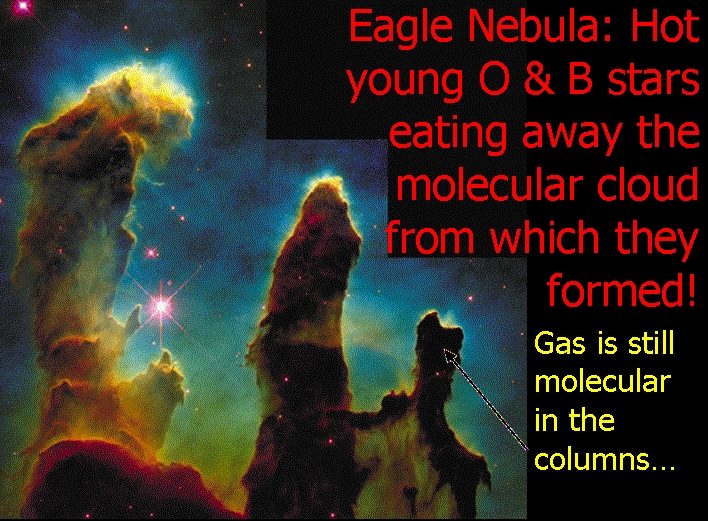
\includegraphics{figures/ISMorion2.jpg}}
\end{center}

\end{minipage}

\begin{minipage}[t]{14cm}
\begin{center}
%{\large \color{red} Interstellar dust }
\end{center}

\end{minipage}}
\vfill 
\end{slide}
%--------------------------------------------------------------------------------------------




%------------------------------------------------------------------------------
\begin{slide}
\begin{center}
\bfseries
{\large {\color{red} Optical Surveys and Stellar Counts}}
\end{center}
\vskip 0.2in
\hrule

\vskip 0.1in
\begin{itemize}
\item {\colour{blue} Hipparcos:} 3,000 stars visible by naked eye
\item {\colour{blue} and many others...} 
\item {\colour{blue} Palomar Observatory Sky Survey:} (first 1950-57, second 1985-1999) 
         photographic, nearly all-sky, 
         two bands, m$<$20.5, astrometric accuracy $\sim$0.5 arcsec, photometric
         accuracy 0.2-0.4 mag (both very non-Gaussian), USNO-B catalog: 10$^9$ sources
\item {\colour{blue} SDSS:} digital, 1/4 sky, 5 bands, m$<$22.5, astrometric accuracy 
        $<$0.1 arcsec absolute,  $\sim$0.02 arcsec relative, photometric
         accuracy 0.02 mag (both nearly Gaussian), several 10$^8$ sources
\end{itemize}
\end{slide}
 
%------------------------------------------------------------------------------
\picslide{figures/stripe_example}{jpg}{}{0.75}{8}{-2.0}{-2.5} 
\Spicslide{figures/M101}{jpg}{Spiralna galaksija}{0.745}{7}{-0.6}{-2.2} 
\Spicslide{figures/UGC03214}{jpg}{UGC03214}{0.585}{7}{-2.1}{-3.2} 
\Spicslide{figures/Segue-4076-3-173_175}{jpg}{}{1.0585}{7}{-0.6}{-2.2} 
%------------------------------------------------------------------------------



%------------------------------------------------------------------------------

\begin{slide}
\begin{center}
{\large \color{red} 
                    Stellar Counts
}
\end{center}

{\color{blue} 
There is a lot of information about the Milky Way structure (and stellar
initial mass function, and stellar evolution) in SDSS imaging data.
}

\vfill
\end{slide}


%------------------------------------------------------------------------------

\begin{slide}
     \begin{center}
        \begin{minipage}{7in}
            \phantom{x} \vskip -2.0in
            \phantom{x} \hskip -0.5in
            {\scalebox{0.9}{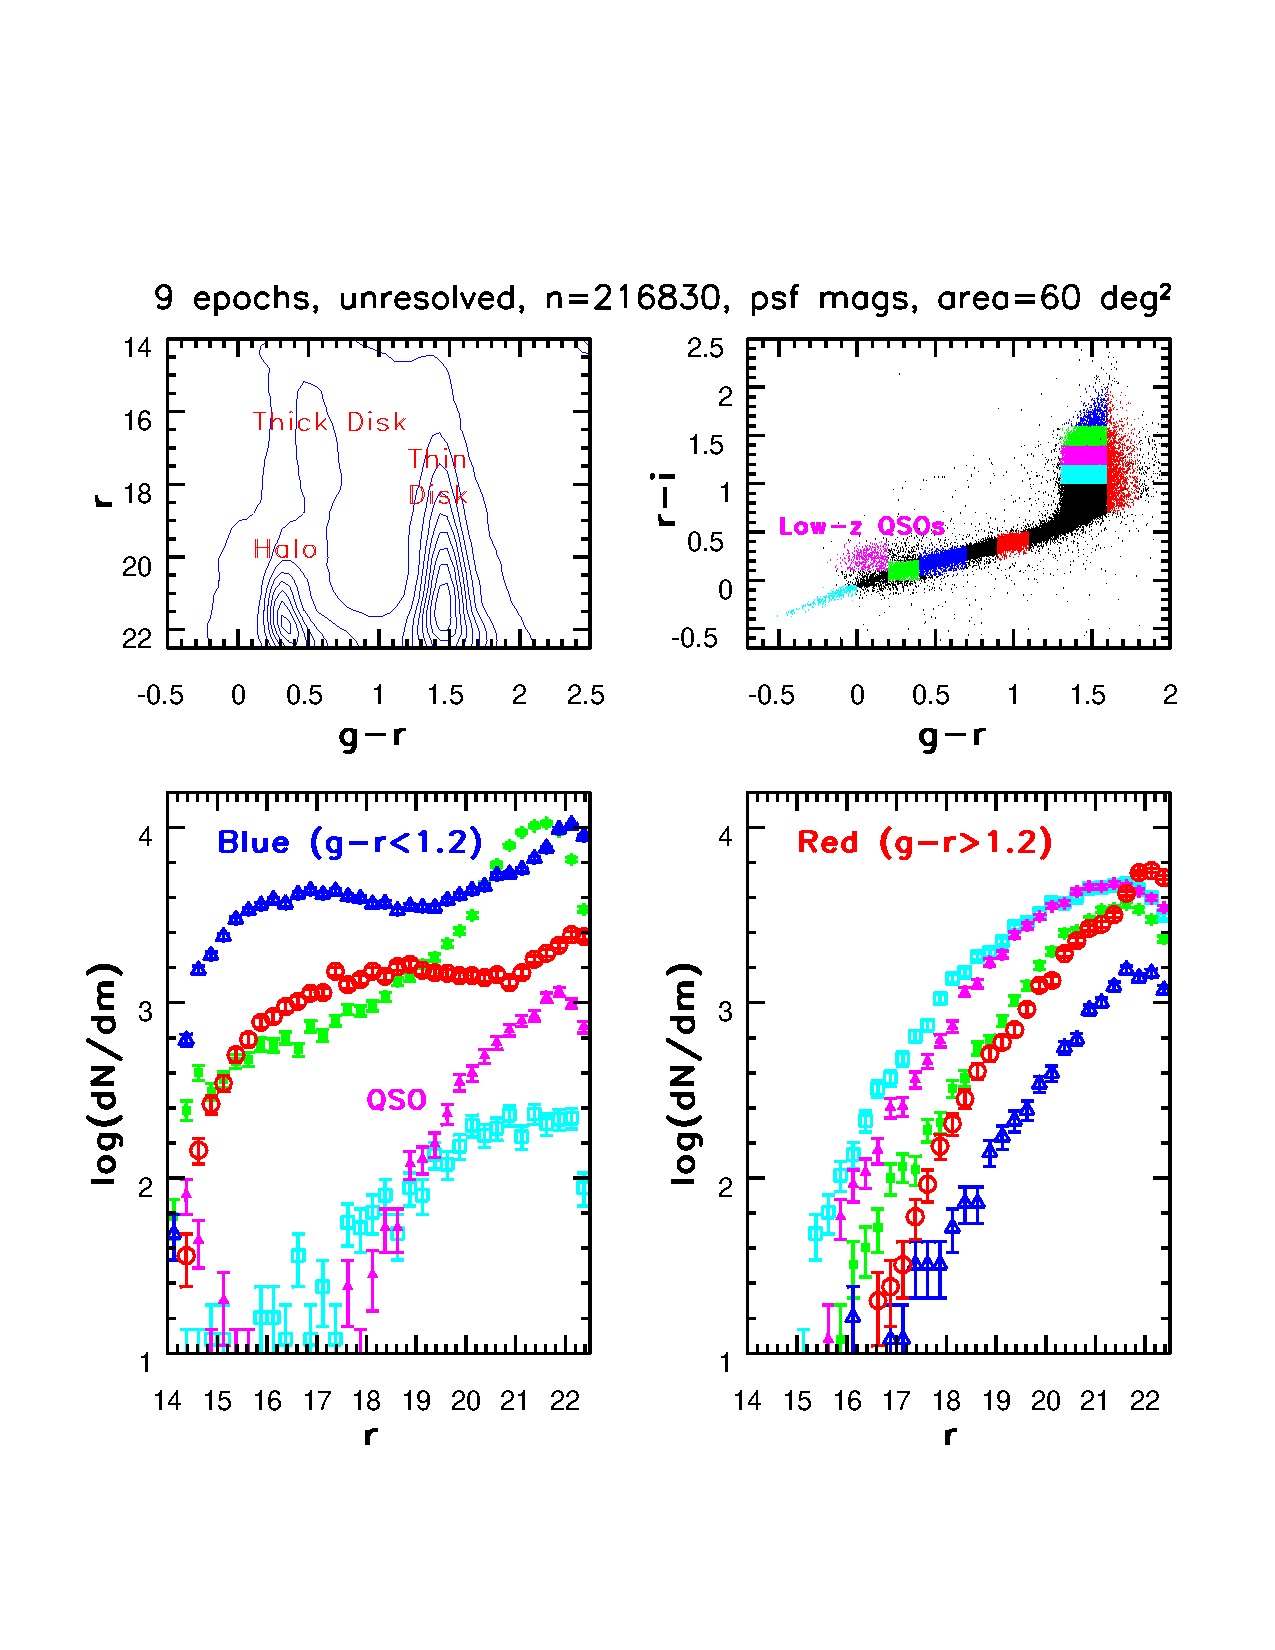
\includegraphics{figures/plotRedLSST.pdf}}}
          %  {\large \color{blue} SDSS unresolved sources}
        \end{minipage}
     \end{center}
     \vfill
\end{slide}


%------------------------------------------------------------------------------


%------------------------------------------------------------------------------

\begin{slide}
\begin{center}
{\large \color{red} 
                    Stellar Counts
}
\end{center}


There is a lot of information about the Milky Way structure (and stellar
initial mass function, and stellar evolution) in SDSS imaging data.

{\color{blue} 
How can we extract and interpret this information? What is the meaning
of local maxima in the differential counts for some (but not all) color
cuts? 
}
     
\vfill
\end{slide}






%------------------------------------------------------------------------------

\begin{slide}
\begin{center}
{\large \color{red}  Computing Differential Stellar Counts $n(m)$  }
\end{center}

\begin{enumerate}

\item
     $n(m) = dN/dm = dN/dV \, dV/dm$, \\ $dN/dV = \rho(l,b,D)$ ($\rho$ constrains Galactic Model)

\item
For a pencil beam: $dV = \Delta \Omega \, D^2 \, dD$

\item
      $D = 10 {\rm pc} \, 10^{0.2(m-M)}$, $dD/dm = 0.2\,ln(10)\, D(m)$

\item
 $n(m) = \rho(l,b,m)\, 0.2\, \Delta \Omega\,ln(10)\,(10\,pc)^3\,10^{-0.6M}\,10^{0.6m}$ \\

{\color{blue} \Large \hskip 1.5in   $n(m) \propto \rho(l,b,m)\, 10^{0.6m}$}

\end{enumerate}  

\vfill
\end{slide}



%------------------------------------------------------------------------------

\begin{slide}
\begin{center}
{\large \color{red}  Examples for $n(m)\propto \rho(l,b,m)\, 10^{0.6m}$ }
\end{center}

\begin{itemize}
\item
{\color{red} Power-law: $ \rho(l,b,D) \propto D^{-n}$} \\

    {\color{blue} \hskip 1.5in    $  n(m) \propto 10^{k\, m}$, $k= 0.6-0.2\,n$}
        \begin{itemize}
         \item
            Euclidian counts (n=0):  $n(m) \propto 10^{0.6\, m}$,
          \item
            Halo counts (n=3):  $n(m) = const.$
       \end{itemize}  
\item 
{\color{red} Exponential disk:  $\rho(l,b,D) \propto e^{-D/H}$} \\
at a distance $D=k\,H$, $n(m)$ has a local slope corresponding to a power-law 
with $n=k$. Hence, for $D=3\,H$, the differential counts for exponential density
distribution have a local maximum! 
\end{itemize}  

\vfill
\end{slide}


%------------------------------------------------------------------------------

\begin{slide}
     \begin{center}
        \begin{minipage}{7in}
            \phantom{x} \vskip -2.0in
            \phantom{x} \hskip -0.5in
            {\scalebox{0.9}{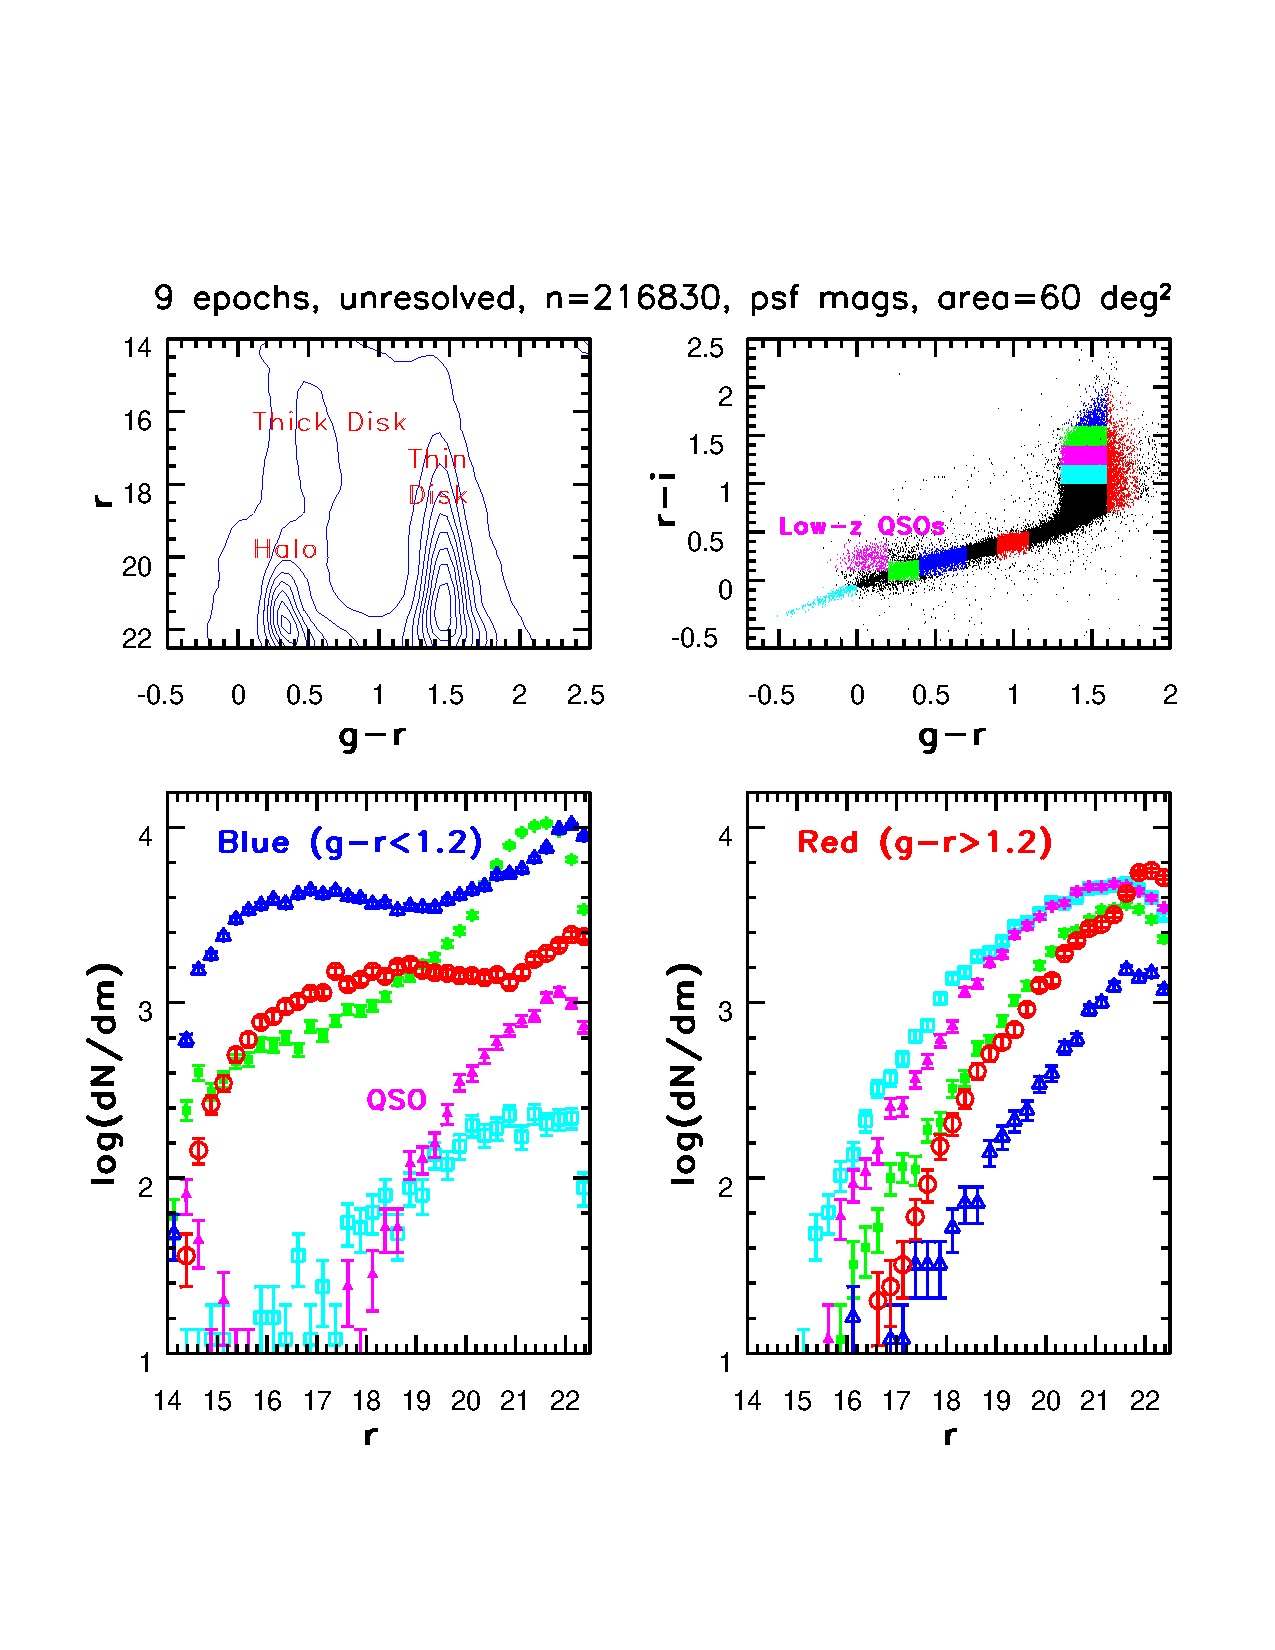
\includegraphics{figures/plotRedLSST.pdf}}}
          %  {\large \color{blue} SDSS unresolved sources}
        \end{minipage}
     \end{center}
     \vfill
\end{slide}


%------------------------------------------------------------------------------


%------------------------------------------------------------------------------
% TWO-SIDED PAGE 
\begin{slide}

\hbox to \hsize{
\begin{minipage}[t]{8cm}
\begin{center}
\vskip -0.8in
\scalebox{0.5}{\hskip -1.6in 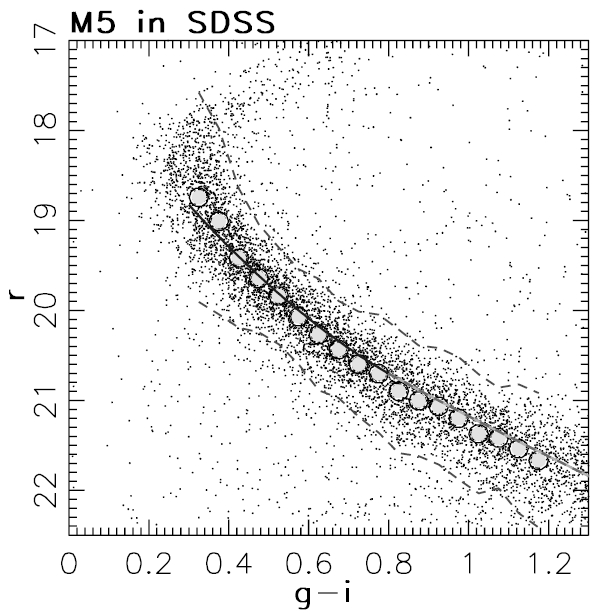
\includegraphics{figures/M5_cmd1.jpg}}
\vskip -0.2in
\scalebox{0.5}{\hskip -2.1in 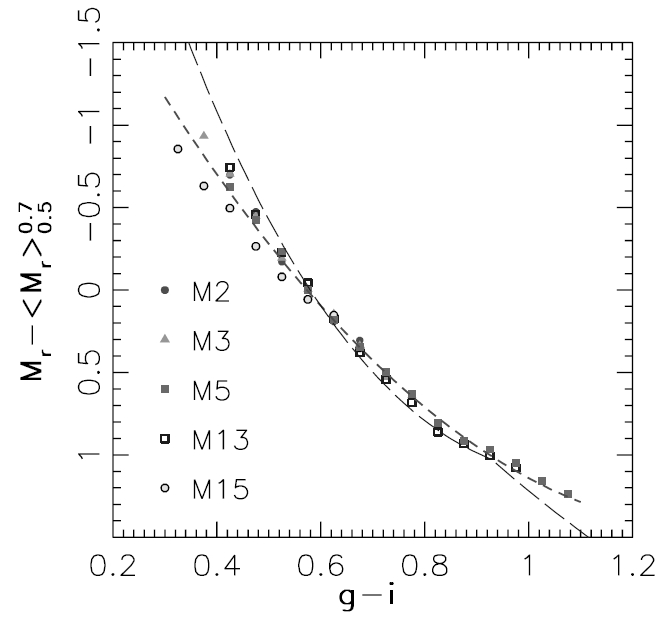
\includegraphics{figures/GCs_cmd1.jpg}}

\end{center}
\end{minipage}

\begin{minipage}[t]{16cm}
\begin{center}
\vskip -1in
{\large \color{red} Photometric Parallax Calibration}
\end{center}


\begin{itemize}
\item {\color{blue} Using a large sample of globular clusters, we can calibrate 
      $M_r(g-i,[Fe/H])$, and then apply it to field stars to get their distances.}
\item {\bf Top Left:} an example of a globular cluster (M5) as observed by
       SDSS; the line is a polynomial fit to the median main sequence (large 
       circles):
\begin{equation}
       M_r = M_r^{0.6} -2.85 + 6.29 \, (g-i) -2.30 \, (g-i)^2  \nonumber
\end{equation}
where $M_r^{0.6}$ is the median absolute magnitude for stars 
with $0.5<g-i<0.7$. 
\item {\bf Bottom Left:} this is a good fit to a number of globular 
  clusters observed by SDSS, showing that the main effect of metallicity
  is to slide the main sequence vertically (i.e. along luminosity axis,
  changing $M_r^{0.6}$), without much effect on its {\it shape}.
\end{itemize}

\end{minipage}}
\vfill 
\end{slide}
%--------------------------------------------------------------------------------------------


%------------------------------------------------------------------------------

\begin{slide}
     \begin{center}
        \begin{minipage}{7in}
            \phantom{x} \vskip  -0.5in
            \phantom{x} \hskip -1.4in
            {\scalebox{1.1}{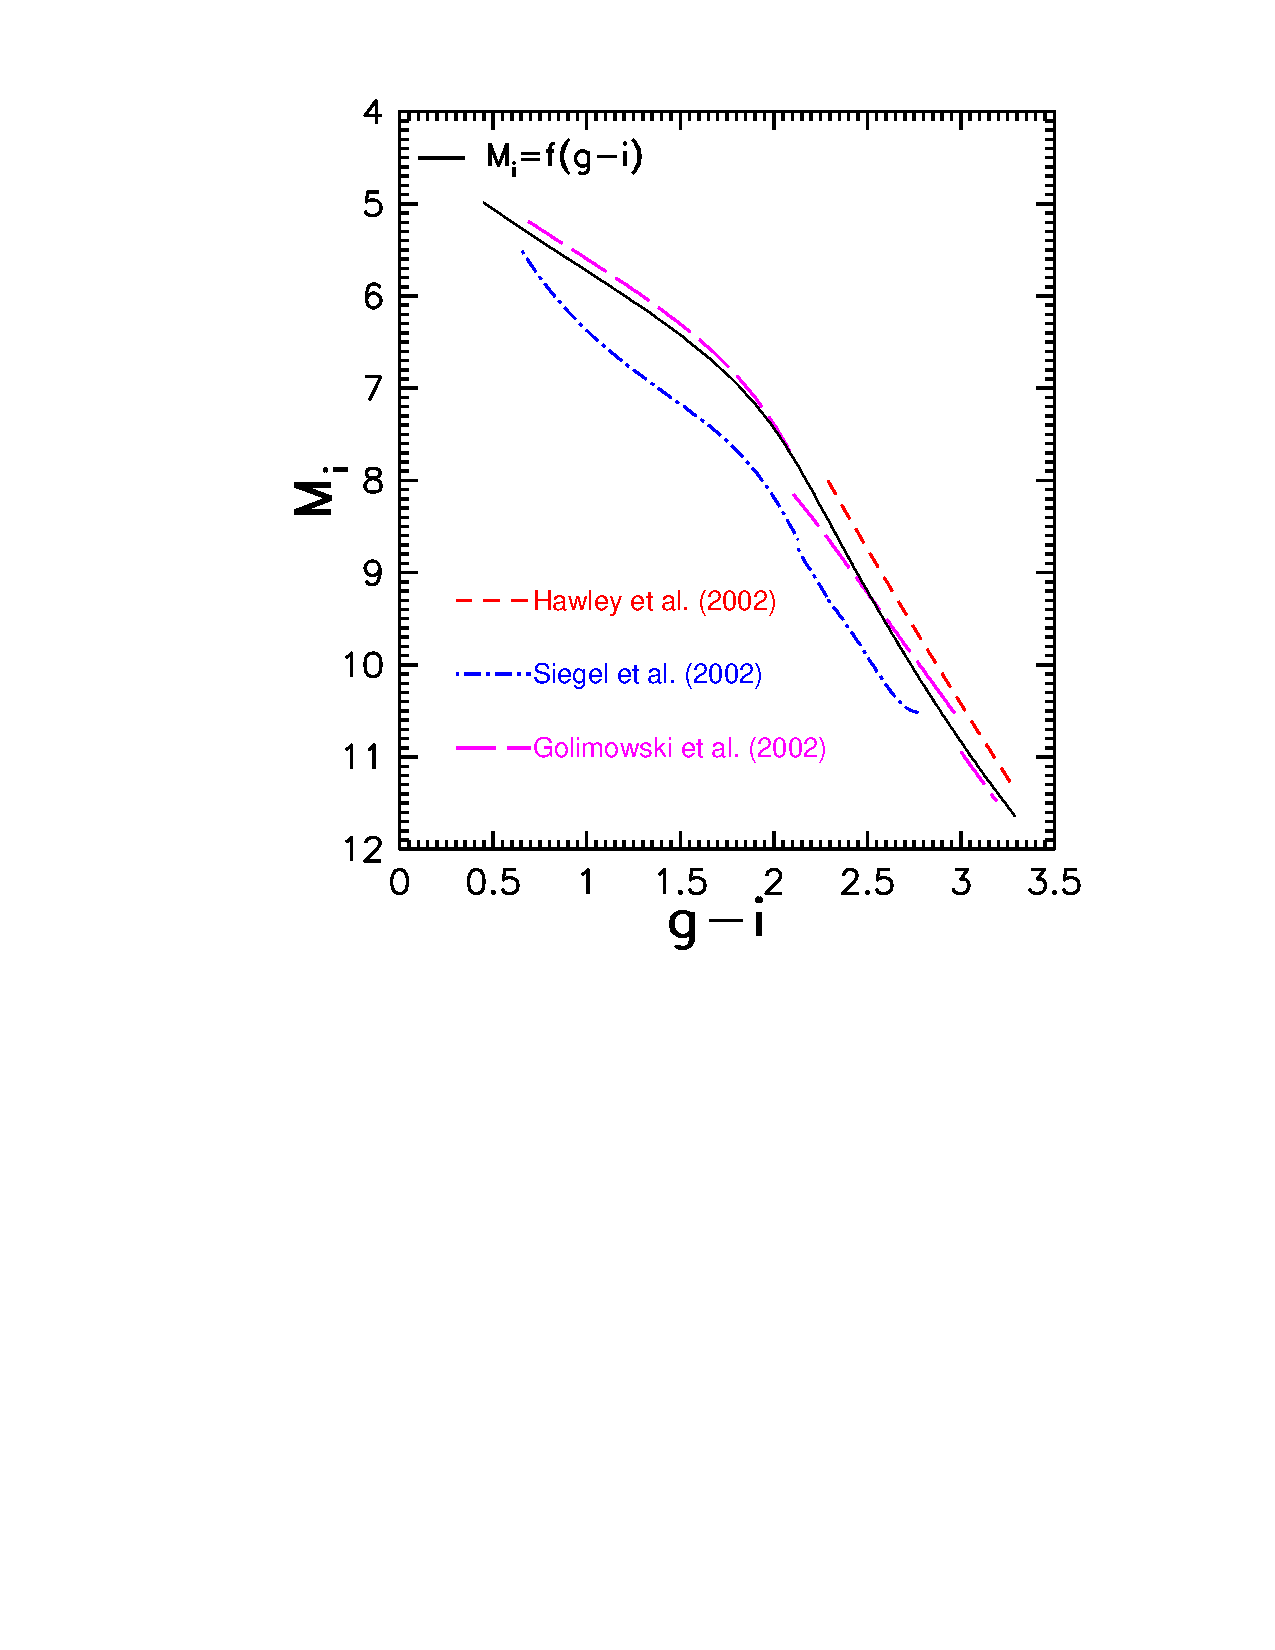
\includegraphics{figures/plotMivsgi.pdf}}}           
        \end{minipage}
     \end{center}
    \vfill
\end{slide}
%------------------------------------------------------------------------------

\begin{slide}
\begin{center}
{\large \color{red}  What are SDSS counts telling us? }
\end{center}

\begin{itemize}
\item
{\color{blue} For $g-r\sim0.5$, maximum for $n(m)$ at $r=17$} \\
    $g-r\sim0.5$ implies $g-i\sim0.8$ and $M_r\sim5.7$: $H'\sim1800 kpc$
\item
{\color{blue} For $r-i\sim1.5$, maximum for $n(m)$ at $r=21.5$} \\
    $r-i\sim1.5$ implies $g-i\sim2.9$ and $M_r\sim12$: $H'\sim800 kpc$

\item
{\color{red} $H' = H/\sin{b} \sim 2\,H$,} in agreement with expectations
for thin ($H\sim300$pc) and thick ($H\sim1.0$kpc) disks.


\item
{\color{blue} With SDSS we can do better than with this standard approach
because {\color{red} the vast majority ($\sim98-99\%$) of detected stars
are on the main sequence.}}
\end{itemize}  
\vfill
\end{slide}


%------------------------------------------------------------------------------
\begin{slide}
\begin{center}
{\large \color{red}  The Local Group }
\end{center}

\begin{itemize}
\item Edwin Hubble introduced ``The Local Group'' classification and assigned a dozen galaxies to
it: Milky Way, Andromeda (M31), M33, LMC, SMC, ... (today there are over 50 known galaxies 
in the Local Group - SDSS played a major role in new discoveries). Andromeda is ~1 Mpc
away (770 kpc), while LMC is 50 kpc away. 

\item The Local Group is about 3 Mpc across, and itself is a part of the larger Virgo Supercluster.

\item The two largest galaxies are Milky Way and Andromeda, and they dominate the total mass. 
A great astro-trivia question is ``What is the third largest galaxy in the Local Group?''  
(the Triangulum Galaxy).

\item Both Milky Way and Andromeda have their own systems of satellite galaxies (that is, they
are gravitationally bound). For Milky Way, the most famous ones are LMC/SMC and 
Sagittarius Dwarf galaxy. 

\end{itemize}  

\begin{center}
 {\scalebox{0.31}{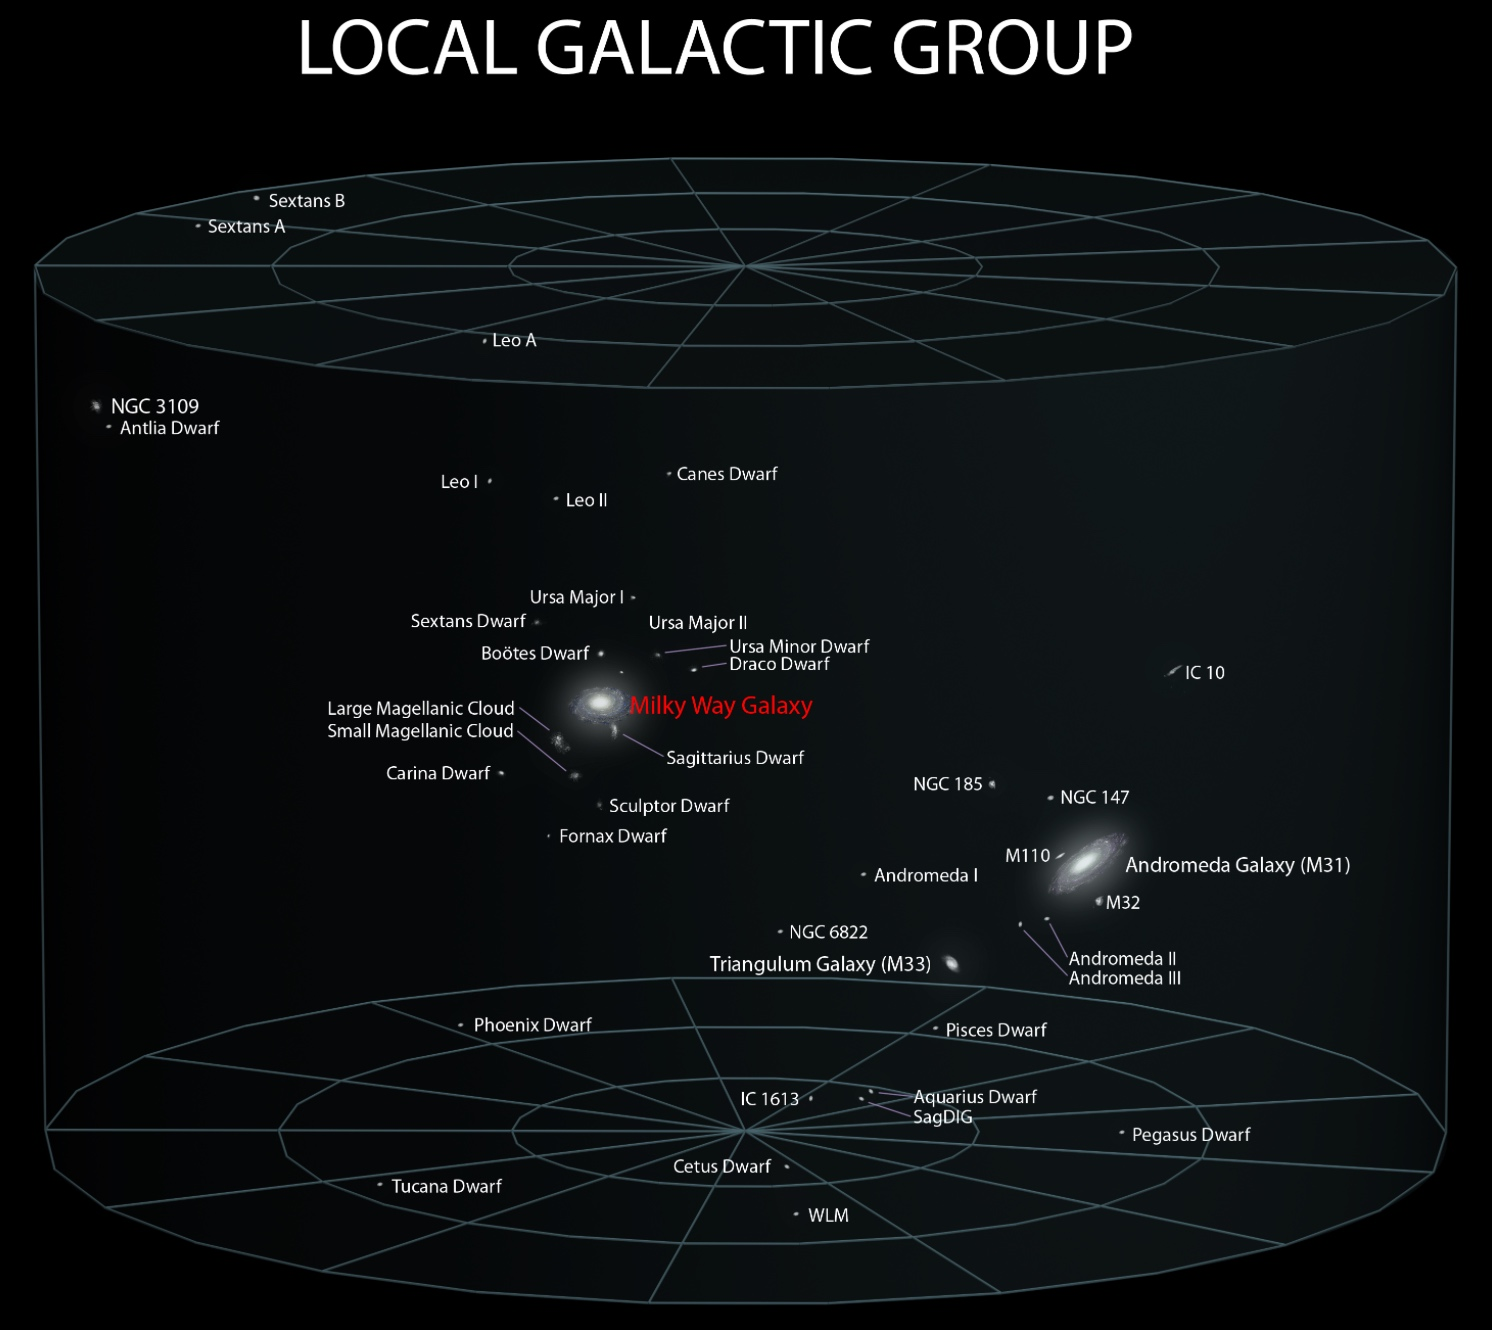
\includegraphics{figures/LocalGroup.jpg}}}     
\end{center}

\vfill
\end{slide}


\end{document} 



